\documentclass[letterpaper,11pt]{report}

\usepackage[utf8]{inputenc}

%idioma
\usepackage[spanish]{babel}
\selectlanguage{spanish}

%Apendice
\usepackage[toc,page]{appendix}

%formato de bibliografia y citas
\usepackage{cite}
%\usepackage{apacite}
 
\usepackage[nottoc]{tocbibind}

\usepackage{etoc}
\usepackage{blindtext}

%Imagenes
\usepackage{graphicx}
\graphicspath{{./images/}}
%\usepackage[font=small,skip=20pt]{caption}
\setlength{\abovecaptionskip}{15pt plus 5pt minus 2pt}

%Espacio de interlineado
\usepackage{setspace}
\thispagestyle{empty}
\doublespacing
%\onehalfspacing

%Tamaño de márgenes
\usepackage[left=1.0in, right=1.0in]{geometry}
\usepackage{layout}
%\usepackage{showframe}
\setlength{\marginparwidth}{0pt}
\setlength{\marginparsep}{0pt}
%\setlength{\textheight}{610pt}

%Colores en el texto
%\usepackage{xcolor}
\usepackage[table]{xcolor}

% Incluir subsubsection en el índice
\setcounter{secnumdepth}{3}
\setcounter{tocdepth}{3}

% Landscape pages on demand
\usepackage{lscape}

% tablas
\usepackage{longtable} % Long tables
\usepackage{rotating} % To display tables in landscape
\usepackage{multirow} % Multirows
\usepackage{tabto}

%Acronyms glossary
\usepackage[counter=section,acronym,nomain]{glossaries}
\makeglossaries
\newacronym{api}{API}{Application Programming Interface}
\newacronym{css}{CSS}{Cascading Style Sheet}
\newacronym{csv}{CSV}{Comma Separated Values}
\newacronym{html}{HTML}{Hypertext Markup Language}
\newacronym{jdbc}{JDBC}{Java Data Base Controller}
\newacronym{jdk}{JDK}{Java Development Kit}
\newacronym{pdf}{PDF}{Portable Document Format}
\newacronym{rest}{REST}{Representational State Transfer}
\newacronym{restful}{RESTFUL}{lo mismo que REST, pero al ful}
\newacronym{soa}{SOA}{Service Oriented Architecture}
\newacronym{url}{URL}{Universal Resource Locator}
\newacronym{xhtml}{XHTML}{Extensible HyperText Markup Language}
\newacronym{xls}{XLS}{Microsoft Excel Spreadsheet}
\newacronym{xml}{XML}{Extensible Markup Language}



\newacronym{utc}{UTC}{Coordinated Universal Time}
\newacronym{adt}{ADT}{Atlantic Daylight Time}
\newacronym{est}{EST}{Eastern Standard Time}
\newacronym{gcd}{GCD}{Greatest Common Divisor}
\newacronym{lcm}{LCM}{Least Common Multiple}


%


\begin{document}
\layout 
\tableofcontents

\chapter{Prefacio}

Given a set of numbers, there are elementary methods to compute 
its \acrlong{gcd}, which is abbreviated \acrshort{gcd}. This process 
is similar to that used for the \acrfull{lcm}.

\rowcolors{2}{gray!25}{white}

\noindent
\begin{longtable}{|p{\dimexpr.1\textwidth}|p{\dimexpr.4\textwidth}|p{\dimexpr.5\textwidth-4\tabcolsep}|}

	\hline
	\textbf{acrshort} & \textbf{acrlong} & \textbf{acrfull}\\
	\hline
	\endfirsthead

	\multicolumn{3}{l}%
	{\textit{Continuación de la página anterior}} \\
	\hline
	\textbf{acrshort} & \textbf{acrlong} & \textbf{acrfull}\\
	\hline
	\endhead

	\hline
	\multicolumn{3}{r}
	{\textit{Continua en la siguiente página}} \\
	\endfoot

	\endlastfoot
\rowcolor{gray!50}
	\acrshort{api} & \acrlong{api} & \acrfull{api} \\
	\acrshort{css} & \acrlong{css} & \acrfull{css} \\
	\acrshort{csv} & \acrlong{csv} & \acrfull{csv} \\
	\acrshort{html} & \acrlong{html} & \acrfull{html} \\
	\acrshort{jdbc} & \acrlong{jdbc} & \acrfull{jdbc} \\
	\acrshort{jdk} & \acrlong{jdk} & \acrfull{jdk} \\
	\acrshort{pdf} & \acrlong{pdf} & \acrfull{pdf} \\
	\acrshort{rest} & \acrlong{rest} & \acrfull{rest} \\
	\acrshort{restful} & \acrlong{restful} & \acrfull{restful} \\
	\acrshort{soa} & \acrlong{soa} & \acrfull{soa} \\
	\acrshort{url} & \acrlong{url} & \acrfull{url} \\
	\acrshort{xhtml} & \acrlong{xhtml} & \acrfull{xhtml} \\
	\acrshort{xls} & \acrlong{xls} & \acrfull{xls} \\
	\acrshort{xml} & \acrlong{xml} & \acrfull{xml} \\
	\hline

	\caption{Tabla de acrónimos}
\end{longtable}


\chapter{Introducción}\label{cap1}

\section{Contexto} \label{sec:intro-contexto}
Todos los institutos de salud pública en México cuentan con proveedores que se encargan de surtir los medicamentos a sus respectivas clínicas y hospitales. El documento digital en el cual se asienta la solicitud de un medicamento es llamada \textit{orden de reposición}; este documento contiene la descripción del medicamento y el lugar en donde es solicitada la entrega del mismo. En particular, el \textit{Instituto} para el cual se realiza este proyecto hace llegar a los proveedores las órdenes de reposición a través de su sistema web llamado \textit{Sistema de Abastecimiento}, dentro del cual el proveedor, a su vez, puede confirmar la recepción de las órdenes de reposición.\\
El proveedor tiene operadores dedicados a interactuar con el \textit{Sistema de Abastecimiento}. Las tareas que debe cumplir el operador del \textit{Sistema de Abastecimiento} son: confirmar la recepción de órdenes de reposición al \textit{Sistema de Abastecimiento}, obtener la información necesaria para cumplir con la entrega del medicamento (Figura \ref{fig:flow-proc-contestar}) y extraer las órdenes de reposición que han sido canceladas (Figura \ref{fig:flow-proc-verificar}), lo cual significa que el \textit{Instituto} ya no requiere el medicamento especificado en la orden de reposición y, de ser entregadas, serán rechazadas.\\
El proveedor realiza dos tipos de procesos:
\begin{enumerate}
\item \textbf{Envío de órdenes de reposición}. Un operador accede al \textit{Sistema de Abastecimiento}, con un usuario y contraseña previamente asignados, posteriormente se dirige a la sección \textit{Contestación a Órdenes de Reposición}, que es donde se muestra un listado con las órdenes de reposición emitidas por el \textit{Instituto} que aún no han sido atendidas. El operador manualmente ingresa en cada orden de reposición los datos requeridos: la cantidad de unidades que enviará, fechas de fabricación y de caducidad. A esto se le conoce como responder la orden reposición.\\
Cuando una orden de reposición ha sido \textit{contestada}, en el listado de órdenes de reposición de la sección \textit{Contestación a Órdenes de Reposición} se muestra la opción de ``enviar''. Aquí el operador selecciona la opción ``enviar'' de cada una de las órdenes de reposición que ha contestado, el \textit{Sistema de Abastecimiento} muestra el formato de acuse de recibo, el operador extrae los datos de interés que se muestran en el acuse y hace una impresión de la pantalla. El flujo descrito anteriormente se muestra en la Figura \ref{fig:flow-proc-contestar}.

\begin{figure}[H]
\centering
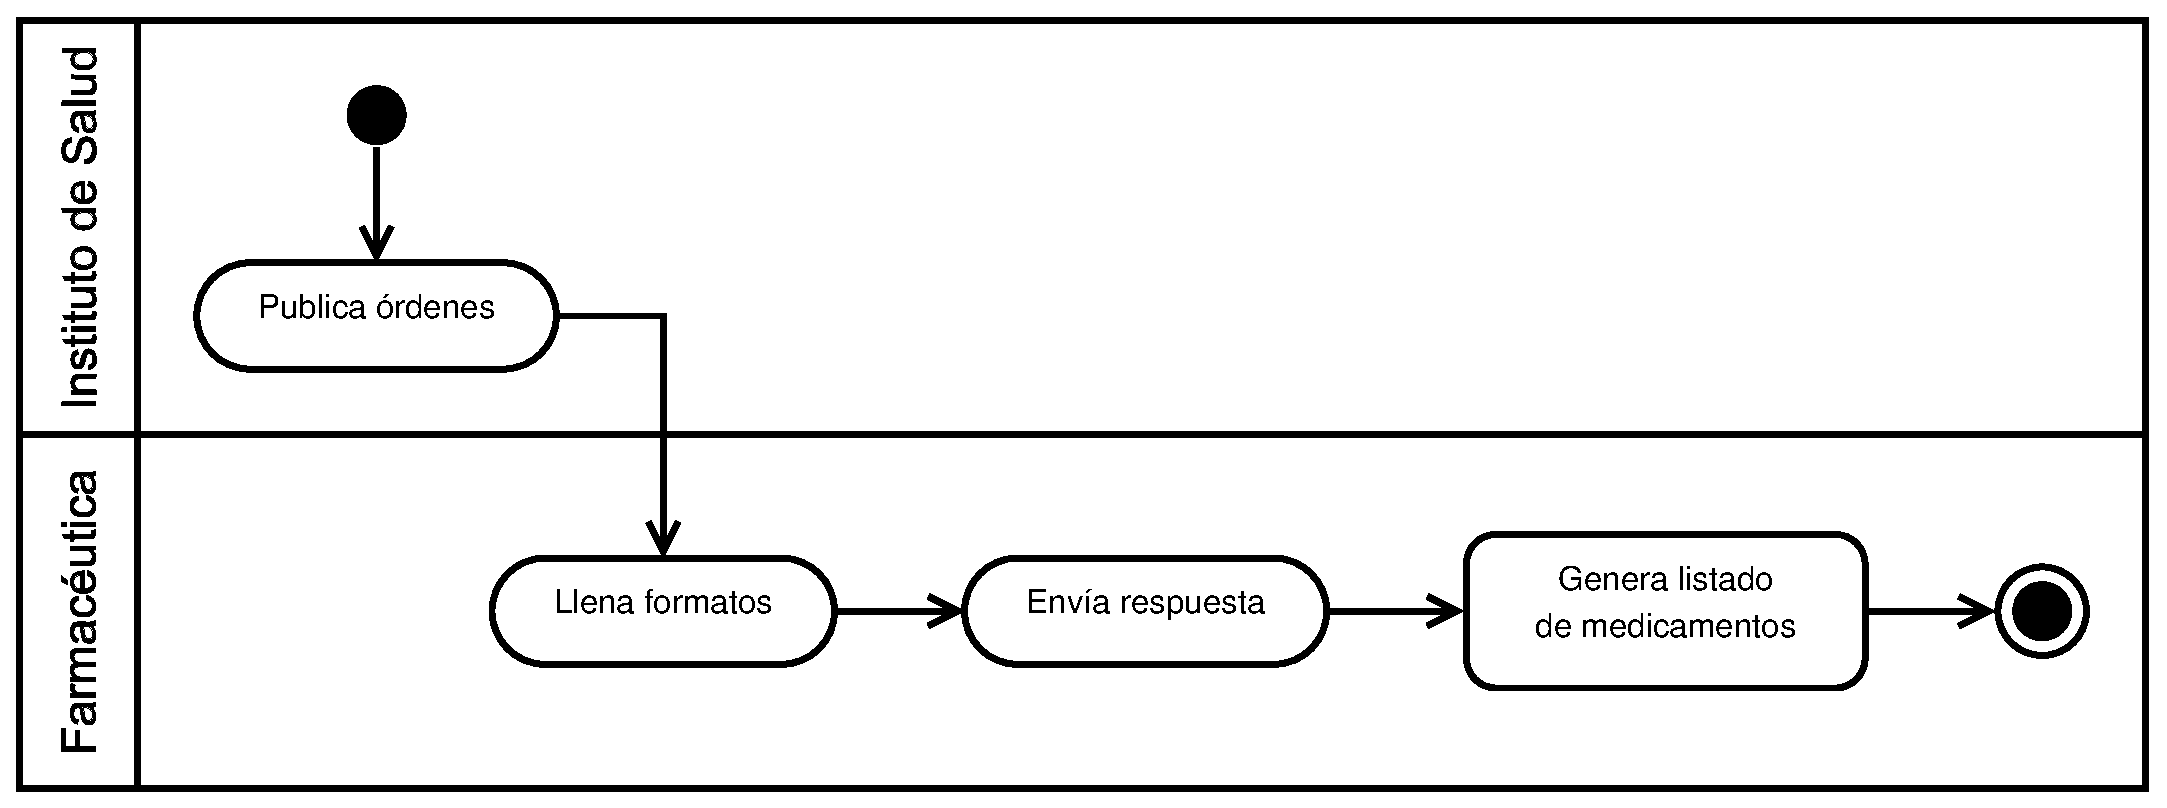
\includegraphics[scale=0.3]{flow-proc-contestar} 
\caption{Flujo del proceso para contestar órdenes de reposición.}
\label{fig:flow-proc-contestar}
\end{figure}

\item \textbf{Verificación de órdenes de reposición canceladas}. Dado que el \textit{Instituto} tiene la facultad de cancelar las órdenes aun cuando ya hayan sido enviadas, es importante para el proveedor evitar el gasto extra que implica retirar medicamento no solicitado que ya ha sido enviado al \textit{Instituto}. El operador accede al \textit{Sistema de Abastecimiento} de la misma manera como se describe en el punto anterior, se dirige a la sección \textit{Consulta de Órdenes}, donde provee información para realizar la búsqueda: rango de fechas de emisión\footnote{Fecha en que la orden fue realizada.}, el estado de la orden como ``cancelada''. Como resultado de esta búsqueda, se muestra un listado con las órdenes que cumplen con tal filtro. El operador copia la lista en un documento en su equipo personal, para posteriormente extraer las órdenes de reposición que han sido canceladas de las cuales no se tenía conocimiento. En la Figura \ref{fig:flow-proc-verificar} se muestra el proceso para verificar las órdenes de reposición canceladas.
\begin{figure}[H]
\centering
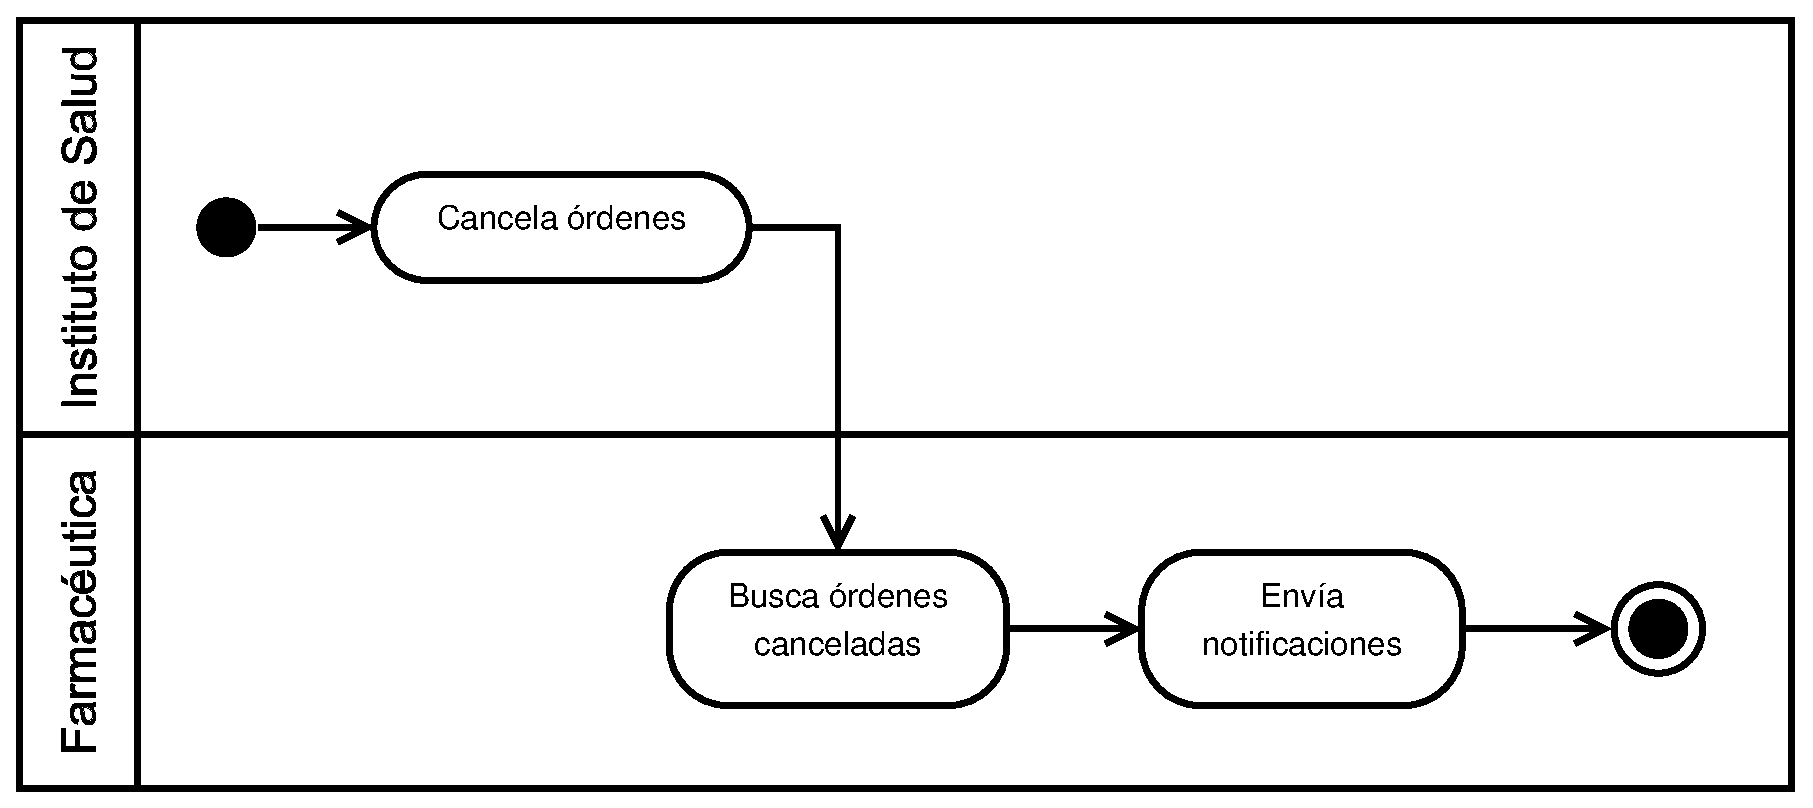
\includegraphics[scale=0.3]{flow-proc-verificar} 
\caption{Flujo del proceso para verificar órdenes de reposición canceladas.}
\label{fig:flow-proc-verificar}
\end{figure}
\end{enumerate}

En este documento se hará referencia de manera indistinta al proveedor\footnote{Quien requiere automatizar la interacción con el Sistema de Abastecimiento para el envío de las órdenes de reposición y la verificación de órdenes canceladas.} como la compañía farmacéutica o simplemente como farmacéutica.\\
Para completar las tareas de envío de órdenes de reposición y verificar las órdenes de reposición canceladas dentro del \textit{Sistema de Abastecimiento}, la farmacéutica dedica diariamente un equipo constituido por tres personas durante toda la jornada laboral. Dependiendo del volumen de órdenes de reposición emitidas por el \textit{Instituto} se puede agregar una persona más al equipo.

\section{Objetivos}
\subsection{Objetivo principal}\label{sec:objetivo-principal}
Describir un sistema de cómputo --de ahora en adelante llamado \textbf{AutoSA}-- que reduzca el tiempo de interacción entre los operadores de la farmacéutica y el \textit{Sistema de Abastecimiento}. Es así que el sistema AutoSA busca cumplir las siguientes metas:
\begin{enumerate}
	\item Reducir el tiempo utilizado para contestar las órdenes de reposición.
	\item Evitar el envío de medicamentos cuyas órdenes de reposición hayan sido canceladas.
	\item Agilizar la generación de reportes sobre las órdenes de reposición atendidas.
\end{enumerate}

\subsection{Objetivos secundarios}\label{sec:objetivos-secundarios}
\begin{enumerate}
\item Reducir el error humano en relación con la manipulación de la información.
\item Ahorrar recursos en la entrega de medicamentos no solicitados.
\item Reducir el tiempo de respuesta a las órdenes de reposición.
\item Dar consistencia en los datos respecto a la generación de reportes estadísticos sobre las órdenes de reposición procesadas.
\end{enumerate}
Por lo anterior, los afiliados del \textit{Instituto} se verán beneficiados pues los medicamentos estarán disponibles con mayor frecuencia en las clínicas y hospitales.

\section{Descripción general de trabajo}\label{sec:desc-general}
La farmacéutica atiende las órdenes de reposición del \textit{Instituto} en el doble de tiempo que su competencia, en particular contestar estas órdenes en el \textit{Sistema de Abastecimiento} requiere diariamente de tres personas dedicadas durante toda la jornada laboral para terminar esta parte del proceso. La solución propuesta para acelerar la respuesta y verificación de órdenes de reposición del \textit{Sistema de Abastecimiento} se encuentra programado por agentes\footnote{Agente dentro de este trabajo se refiere a las rutinas que automatizan los procesos realizados por los operadores del \textit{Sistema de Abastecimiento}.}. Cada agente se dedica a emular las acciones del operador de la farmacéutica, el cual es el responsable de contestar o verificar las órdenes de reposición. El sistema AutoSA cuenta con una base de datos donde se almacenan los datos capturados por los agentes durante la respuesta de órdenes y una interfaz gráfica donde los trabajadores de la farmacéutica puedan realizar tareas de administración. Estas tareas pueden ser: la búsqueda, la edición de órdenes de reposición y la generación de reportes de las órdenes atendidas por los agentes.\\
La automatización de los procesos (Figuras \ref{fig:flow-proc-contestar} y \ref{fig:flow-proc-verificar}) antes mencionados pronostica una reducción de costos por devolución de medicamento no solicitado para el cliente y también la disminución de pérdidas en las ventas por solicitudes no atendidas en los rangos de tiempo acordados con el comprador. Dado lo anterior, se plantea un proyecto de software que cubra las necesidades de automatización y pueda ser administrado por usuarios no especializados en computación.\\
Para resolver el desarrollo del proyecto, el sistema AutoSA se divide en módulos con funcionalidades específicas que se muestran a continuación:
% espaciado
%\pagebreak
% espaciado
\begin{enumerate}
\item \textbf{Automatización de interacción con el Sistema de Abastecimiento}. La automatización de la interacción con el \textit{Sistema de Abastecimiento} consiste en replicar los pasos que sigue el operador de la farmacéutica en el llenado y extracción de información de las órdenes de reposición del \textit{Sistema de Abastecimiento}, es decir, listar los pasos que sigue el operador cuando contesta las órdenes de reposición; describir las reglas de negocio necesarios para llenar los formularios que presenta el \textit{Sistema de Abastecimiento} al responder una orden de reposición; por último, se identifican las fuentes de los datos que se ocupan para llenar tales formularios y se define la forma de almacenamiento de la información necesaria de cada formulario.
\item \textbf{Generación de reportes}. La generación de reportes consiste en plasmar la información obtenida de las órdenes de reposición contestadas en el módulo anterior. La farmacéutica tiene ya una plantilla que se utiliza para pasar los pedidos a otras áreas, con el fin de continuar la atención de las órdenes de reposición; además de obtener estadísticas relacionadas con la cantidad de órdenes de reposición atendidas y canceladas.
\item \textbf{Interfaz de usuario}. La interfaz de usuario se refiere a la aplicación que muestra una interfaz gráfica en la cual los operadores de la farmacéutica pueden solicitar la generación de reportes, hacer consultas y modificaciones a las órdenes de reposición atendidas por el primer módulo.
\end{enumerate}

\subsection{Arquitectura de la solución}
Una definición de arquitectura de software es dada por Bourque\cite{SWEBOOK}:
\begin{quote}
El conjunto de estructuras necesarias para la comprensión de un sistema en el cual se comprometen elementos de software, relaciones entre ellos y sus propiedades.
\end{quote}
Esta definición expone que los requerimientos del cliente se traducen en especificaciones técnicas para los desarrolladores. Aplicando la definición anterior al presente proyecto donde tenemos los siguientes componentes (Figura \ref{fig:dia-package-small}):
\begin{figure}[h]
\centering
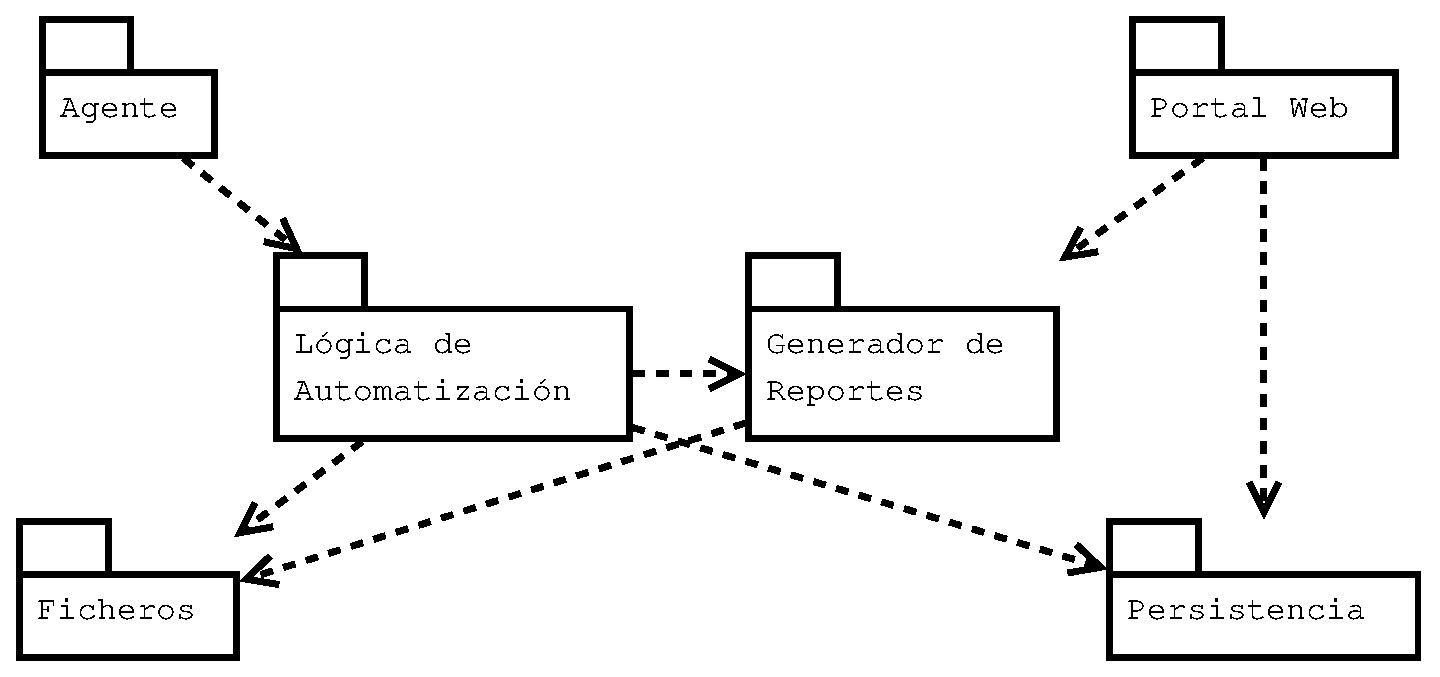
\includegraphics[scale=0.5]{dia-package-small} 
\caption{Módulos de la arquitectura.}
\label{fig:dia-package-small}
\end{figure}
% espaciado
%\pagebreak
% espaciado
\begin{itemize}
\item \textbf{Agente (robot)}. Interactúa directamente con el \textit{Sistema de Abastecimiento}, es el componente que automatiza las acciones de los operadores humanos de la farmacéutica.
\item \textbf{Lógica de Automatización}. Son bibliotecas y rutinas que se encargan de prestar los servicios necesarios al agente para su funcionamiento. Permite comunicación con la base de datos, guarda las capturas de pantalla en el sistema de archivos y provee la configuración de inicio al agente.
\item \textbf{Persistencia}. Es el componente que se encarga de llevar la persistencia de los datos obtenidos durante la respuesta a las órdenes de reposición.
\item \textbf{Ficheros}. Este componente es el encargado de manejar operaciones con el sistema de archivos para almacenar las capturas de pantalla al momento de enviar la respuesta de cada orden de reposición.
\item \textbf{Generador de Reportes}. Este módulo está encargado de la generación de reportes, tales como: órdenes de reposición atendidas, canceladas y formatos de órdenes de reposición enviadas.
\item \textbf{Portal Web}. Portal mediante el cual los usuarios pueden hacer correcciones a los datos obtenidos de las órdenes de reposición, reimprimir el formato de envío de la orden de reposición  y descargar los reportes generados por el módulo generador de reportes.
\end{itemize}
% espaciado
%\pagebreak
% espaciado
\subsection{Metodología utilizada}
El proyecto es abordado con la metodología \textit{Scrum}, la cual es un marco de trabajo para desarrollar, entregar y mantener productos complejos. Ésta consiste en un conjunto de roles, eventos, artefactos y reglas que los ligan. \textit{Scrum} da un enfoque adaptivo mientras promueve la entrega continua de soluciones y divide el desarrollo en ventanas de tiempo llamadas \textit{sprint}\cite{scrum}.\\
Dentro de \textit{Scrum} destacan los siguientes roles utilizados para el desarrollo del proyecto AutoSA\cite{scrum}:
\begin{itemize}
	\item \textit{Product Owner}: es responsable de maximizar el valor del producto que resulta del trabajo del \textit{Development Team}. Es la persona encargada de mantener el conjunto de tareas pendientes para futuros \textit{sprints}.
	\item \textit{Development Team}: es un grupo de profesionales encargado de realizar el trabajo necesario para completar las entregas de cada \textit{sprint}.
	\item \textit{Scrum Master}: es la persona responsable de promover y soportar \textit{Scrum} como está definido en la guía de \textit{Scrum}. Es un líder servil para el \textit{Scrum Team} que auxilia a este último a maximizar el valor del producto creado y ayuda a los involucrados en el desarrollo a comprender \textit{Scrum}.
	\item \textit{Scrum Team}: es conformado por el \textit{Product Owner}, el \textit{Development Team} y el \textit{Scrum Master}. \textit{Scrum Team} es un equipo de trabajo autoorganizado y multifuncional. Está diseñado para optimizar la flexibilidad, creatividad y productividad sin depender de personas ajenas al equipo.
	\item \textit{Stakeholder}: esta definición proviene directamente de su significado en inglés, refiere a las personas que tienen interés en el producto.
\end{itemize}
El grupo de trabajo (\textit{Scrum Team}) formado por la consultora para el proyecto AutoSA consta de dos personas:
\begin{enumerate}
	\item Desarrollador: es la persona que cumple con las funciones siguientes:
	\begin{enumerate}
		\item Levantar los requerimientos de los \textit{stakeholders} de la farmacéutica.
		\item Cumplir con el rol de \textit{Product Owner} al ser encargado de mantener la lista de tareas para los \textit{sprints} futuros.
		\item Hacer investigación sobre tecnologías adecuadas para el desarrollo.
		\item Realizar el diseño e implementación de los componentes del sistema AutoSA.
		\item Formar parte del \textit{Scrum Team}.
	\end{enumerate}
	\item Arquitecto: tiene las siguientes responsabilidades:
	\begin{enumerate}
		\item Supervisar y aprobar el diseño e implementación realizado por el desarrollador.
		\item Hacer investigación sobre tecnologías adecuadas para el desarrollo.
		\item Cumplir con el rol de \textit{Scrum Master}.
		\item Formar parte del \textit{Scrum Team}.
	\end{enumerate}
\end{enumerate}
El proyecto fue planeado para ser realizado de julio a diciembre de 2014. Su conclusión es la liberación del sistema AutoSA que consiste en el despliegue total de los módulos en el ambiente productivo provisto por la farmacéutica dando como resultado los siguientes productos:
\begin{itemize}
\item Rutinas para la generación de objetos en base de datos.
\item Rutinas para la creación de la estructura de directorios en el sistema de archivos.
\item Archivos de configuración propios de cada módulo.
\item Herramienta y rutinas de automatización.
\item Bibliotecas del portal web.
\item Manual de instalación y de usuario.
\item Capacitación a usuarios finales.
\end{itemize}
El autor del presente documento cumplió con rol de desarrollador desde el inicio del proyecto AutoSA hasta su liberación.

\section{Resumen}
El \textit{Instituto de Salud}, mediante su \textit{Sistema de Abastecimiento}, realiza las órdenes de reposición de medicamentos a las farmacéuticas. Estas últimas invierten veinticuatro horas hombre por día para lograr contestar todas las órdenes de reposición. Reducir el tiempo en que se contestan las órdenes de reposición aumenta la velocidad de respuesta de la farmacéutica para entregar los medicamentos a centros de salud del \textit{Instituto}, motivo por el cual le interesa automatizar esta parte. El sistema AutoSA que se propone en este documento da solución mediante dos subsistemas: uno que automatiza los procedimientos de interacción con el \textit{Sistema de Abastecimiento} y otro que permite al personal de la farmacéutica generar reportes y acceder a datos de las órdenes de reposición atendidas.

\renewcommand{\appendixname}{Apéndice}
\renewcommand{\appendixtocname}{Apéndices}
\renewcommand{\appendixpagename}{Apéndices}
\begin{appendices}
\chapter{Lenguaje de Modelado Unificado}

El Lenguaje de Modelado Unificado (nombrado en inglés \textit{Unified Modeling Language}, UML) permite la representación de una amplia variedad de aspectos de sistemas de software como lo son requerimientos, casos de uso, estructuras de datos, procesos\cite{UMLClassroom}. En este apéndice se mostrarán los diagramas que se han utilizado en este documento, así mismo nada más se hará mención de la notación utilizada.

\section{Diagrama de casos de uso}\label{sec:uml-cu}
El diagrama de casos de uso es un modelo de los requerimientos de un sistema a alto nivel, estos requerimientos se describen gráficamente en escenarios (o cosos de uso) que se muestran a través de un diagrama\cite{UMLClassroom, SoftwareEngineeringUML}.\\
Un diagrama de casos uso utiliza la siguiente notación\cite{UMLClassroom, SoftwareEngineeringUML} (ver Figura \ref{fig:uml-nota-use-case}):
\begin{enumerate}
  \item \textbf{Actor}: es una persona o sistema externo que interactúa con el sistema, se representa con un muñeco de líneas.
  \item \textbf{Caso de uso}: describe una funcionalidad del sistema, se representa con una elipse.
  \item \textbf{Límites del sistema}: separa a los actores de los casos de uso, se representa con un rectángulo.
  \item \textbf{Asociación}: representa la interacción de un actor con el caso de uso, se representa como una línea continua.
  \item \textbf{Inclusión}: indica dependencia entre casos de uso, se representa con una flecha de línea de guiones.
\end{enumerate}

\begin{figure}[h]
  \centering
  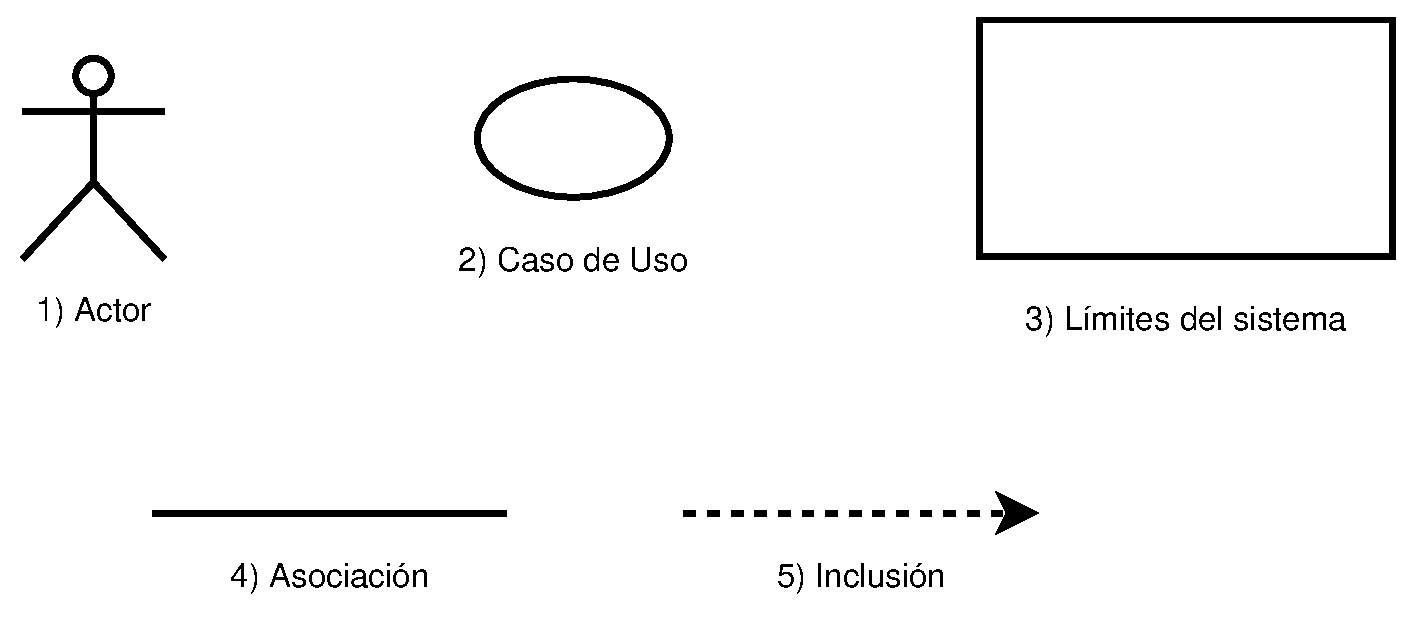
\includegraphics[scale=0.5]{uml-nota-use-case}
  \caption{Notación para diagramas de caso de uso\cite{SoftwareEngineeringUML}.}
  \label{fig:uml-nota-use-case}
\end{figure}

\section{Diagrama de actividad}\label{sec:uml-act}
Un diagrama de actividad modela el flujo de un proceso dentro del sistema, se compone de actividades y muestra las transiciones entre ellas, también puede ser utilizado para modelar la lógica de negocio\cite{UMLClassroom, SoftwareEngineeringUML}.\\
Un diagrama de actividad utiliza la siguiente notación\cite{UMLClassroom, SoftwareEngineeringUML} (ver Figura \ref{fig:uml-nota-activity}):
\begin{enumerate}
  \item \textbf{Inicio}: indica el inicio del flujo, se representa con un círculo.
  \item \textbf{Fin}: indica el fin del flujo, se presenta con un círculo dentro de una circunferencia, concéntricos.
  \item \textbf{Actividad}: es una acción dentro del diagrama, se representa con un rectángulo de esquinas redondeadas.
  \item \textbf{Flujo}: indica la secuencia entre actividades, se representa con una flecha.
  \item \textbf{Decisión}: es una bifurcación del flujo que depende de una condición, se representa con un rombo o diamante.
  \item \textbf{Conjunción}: es la unión entre flujos del diagrama, se representa con una barra rectangular.
  \item \textbf{Notas}: son observaciones a ciertos aspectos del diagrama\footnote{Este símbolo es utilizado en todos los diagramas UML}, se representa con un rectángulo que tiene un triángulo en la esquina superior derecha.
  \item \textbf{Partición}: indica la ejecución de actividades del sistema por parte de componentes del sistema o actores, se representa con con un rectángulo que contiene actividades y en el encabezado el identificador del componente o actor.
\end{enumerate}

\begin{figure}[h]
  \centering
  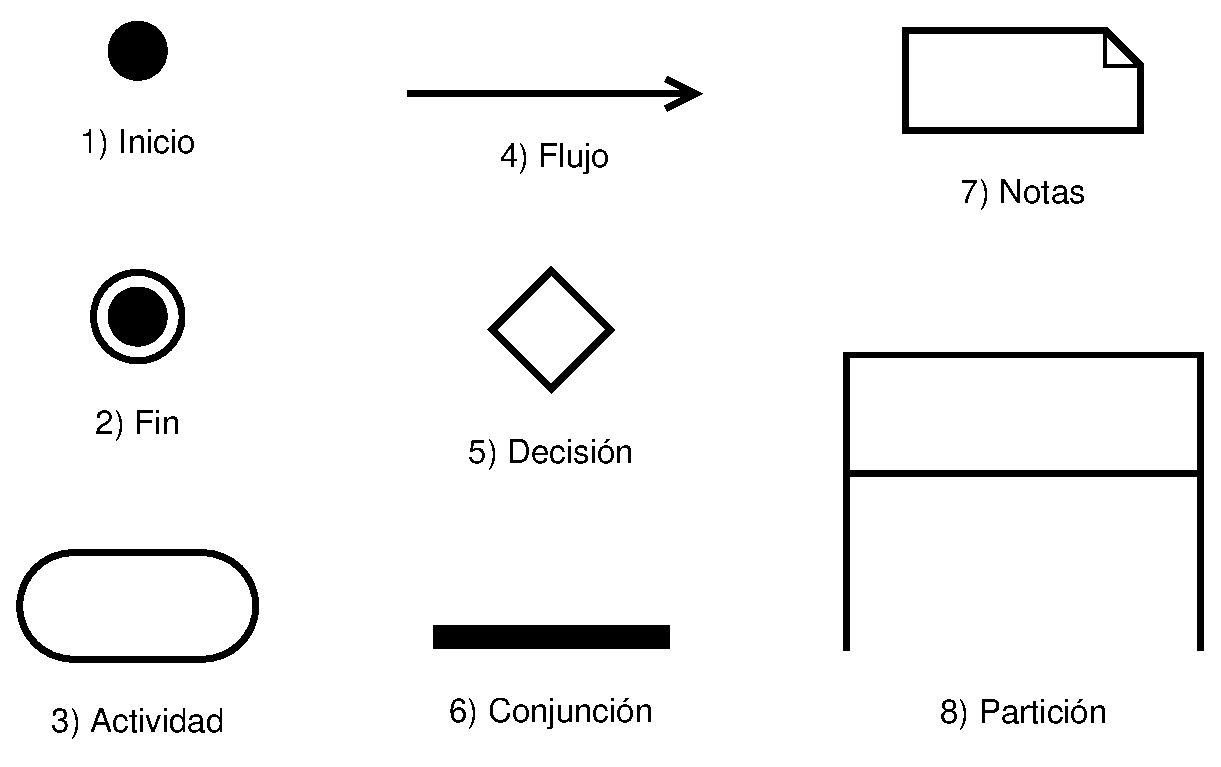
\includegraphics[scale=0.5]{uml-nota-activity}
  \caption{Notación para diagramas de actividad\cite{SoftwareEngineeringUML}.}
  \label{fig:uml-nota-activity}
\end{figure}

\section{Diagrama de componentes}\label{sec:uml-comp}
Un diagrama de componentes es la representación del sistema en unidades independientes del sistema\cite{UMLClassroom, SoftwareEngineeringUML}.\\
Un diagrama de actividad utiliza la siguiente notación\cite{UMLClassroom, SoftwareEngineeringUML} (ver Figura \ref{fig:uml-nota-component}):
\begin{enumerate}
  \item \textbf{Componente}: es una pieza independiente del sistema que provee servicios (interfaces) y consume servicios de otros componentes, se representa como un rectángulo con dos rectángulos más pequeños en columna superpuestos del lado izquierdo.
  \item \textbf{Interfaz}: es un conjunto de operaciones que ofrece el componente, se representa con un una circunferencia y una línea que une a la circunferencia con el componente.
  \item \textbf{Acoplamiento}: indica el consumo de una interfaz, se representa con media circunferencia que envuelve a una interfaz y se conecta al componente con una línea continua.
\end{enumerate}

\begin{figure}[h]
  \centering
  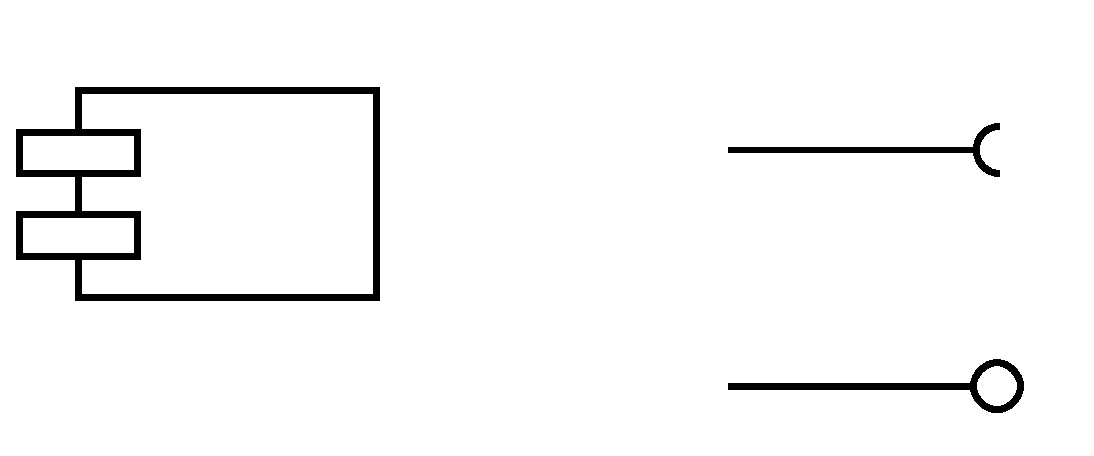
\includegraphics[scale=0.5]{uml-nota-component}
  \caption{Notación para diagramas de secuencia\cite{SoftwareEngineeringUML}.}
  \label{fig:uml-nota-component}
\end{figure}

\section{Diagrama de secuencia}\label{sec:uml-seq}
Un diagrama de secuencia describe las interacciones entre objetos para realizar una tarea, resalta la cronología de mensajes entre objetos así como la creación de éstos\cite{UMLClassroom, SoftwareEngineeringUML}.\\
Un diagrama de secuencia utiliza la siguiente notación\cite{UMLClassroom, SoftwareEngineeringUML} (ver Figura \ref{fig:uml-nota-sequence}):
\begin{enumerate}
  \item \textbf{Actor}: ver descripción de \ref{sec:uml-cu}.
  \item \textbf{Objeto}: es una parte del sistema que puede representar un rol, clase, componente o actor, se representa con un rectángulo con el nombre del objeto subrayado.
  \item \textbf{Mensaje}: es la comunicación entre dos objetos, se representa con una flecha de línea continua y tiene la descripción del mensaje.
  \item \textbf{Mensaje de retorno}: es un mensaje (en sentido contrario) que da respuesta a un mensaje anterior, se representa con una flecha de línea de guiones y tiene la descripción del contenido del mensaje.
  \item \textbf{Bloque}: es un conjunto de mensajes unidos bajo una estructura de control, se representa con un rectángulo que delimita una secuencia de mensajes y en la parte superior izquierda tiene la descripción del control de flujo dentro de un rectángulo.
  \item \textbf{Foco de control}: indica el tiempo que el objeto está activo durante el flujo, se representa como una barra vertical.
  \item \textbf{Línea de tiempo}: sirve como referencia de tiempo, es una línea punteada vertical que acompaña a un foco de control.
\end{enumerate}

\begin{figure}[h]
  \centering
  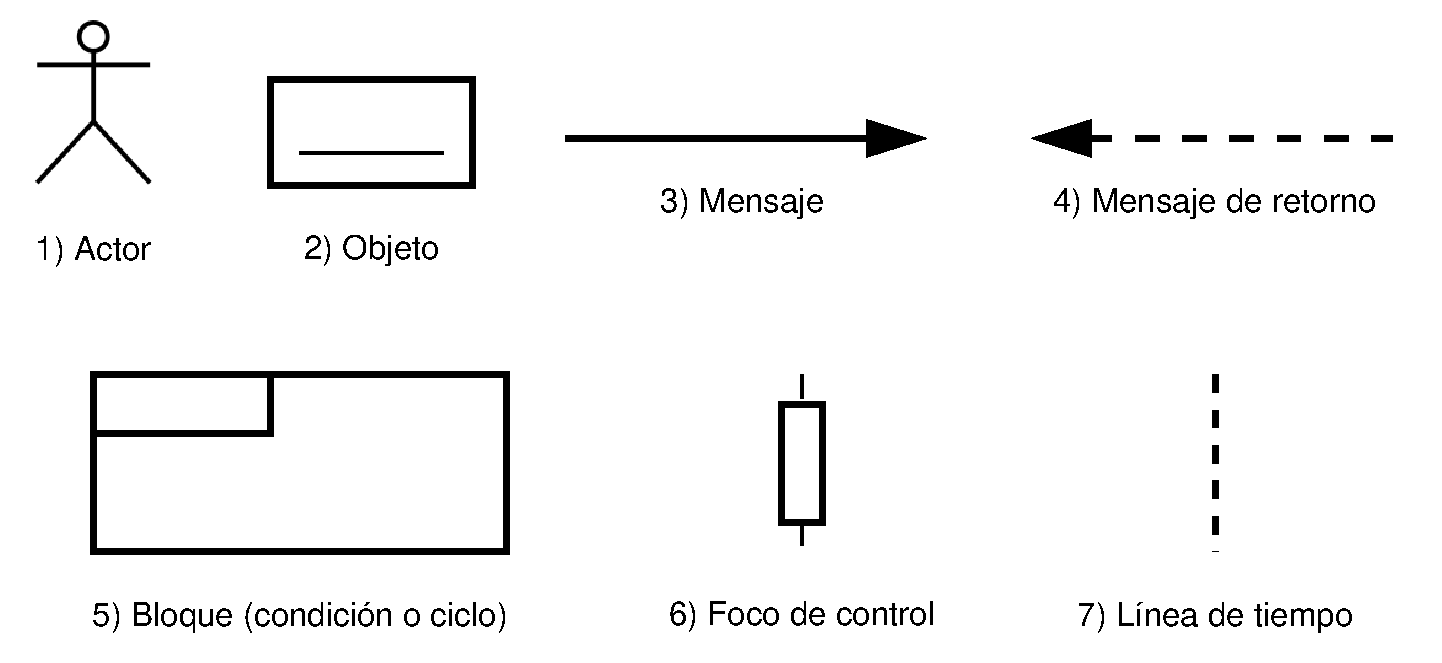
\includegraphics[scale=0.5]{uml-nota-sequence}
  \caption{Notación para diagramas de secuencia\cite{SoftwareEngineeringUML}.}
  \label{fig:uml-nota-sequence}
\end{figure}


\section{Diagrama de clases}\label{sec:uml-class}
Una diagrama de clase, como su nombre lo indica, representa la estructura y relaciones que tiene una clase\cite{UMLClassroom, SoftwareEngineeringUML}.\\
Un diagrama de clase utiliza la siguiente notación\cite{UMLClassroom, SoftwareEngineeringUML} (ver Figura \ref{fig:uml-nota-class}):
\begin{enumerate}
  \item \textbf{Clase}: es un rectángulo dividido en tres secciones horizontales:
  \begin{enumerate}
     \item[1.] \textbf{Nombre}: nombre de la clase, la tipografía normal es con letras gruesas, si se utilizan letras delgadas indica que se trata de un tipo de dato abstracto. 
     \item[2.] \textbf{Atributos}: son los atributos de la clase, se presentan en formato \textit{[nombre]:[tipo]}; al inicio se incluye el alcance:
     \begin{itemize}
       \item [+] público.
       \item [\#] protegido.
       \item [-] privado.
     \end{itemize}
     \item[3.] \textbf{Métodos}: métodos de la clase, descripción similar a los atributos salvo que después del nombre se escriben los parámetros entre paréntesis:
     \begin{center}
       \textit{[alcance] [nombre]([[nombre parámetro]: [tipo parámetro]]*): [tipo]}
     \end{center}
   \end{enumerate} 
  \item \textbf{Clase sin atributos}: similar al punto 1, pero no contiene la sección de atributos.
  \item \textbf{Herencia}: es una flecha con punta cerrada, la dirección de la flecha indica la clase de cual se hereda.
  \item \textbf{Composición}: es una flecha con punta en rombo, indica que una clase contiene referencia a otra clase.
\end{enumerate}

\begin{figure}[h]
  \centering
  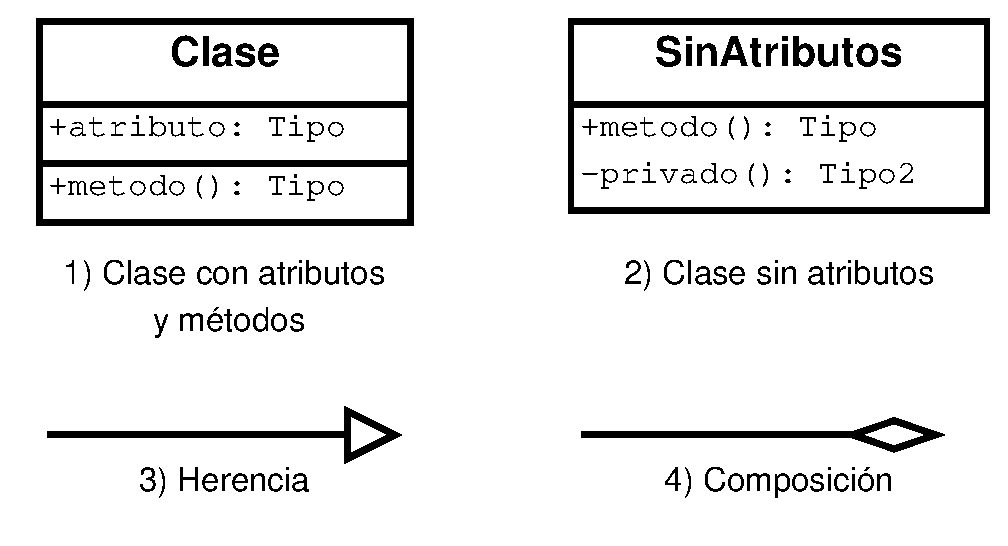
\includegraphics[scale=0.5]{uml-nota-class}
  \caption{Notación para diagramas de clase\cite{SoftwareEngineeringUML}.}
  \label{fig:uml-nota-class}
\end{figure}

\chapter{Técnicas de Diseño}\label{sec-patrones}

\section{Patrones de Diseño}
``Un patrón describe un problema recurrente sobre un ambiente, y entonces describe la técnica que soluciona el problema de forma tal que puede ser utilizado sobre cualquier instancia del problema''\cite{DesignPatterns}, es decir, que dados los requerimientos funcionales del sistema es posible analizar la comunicación entre sus distintas partes y de esta forma saber lo patrones que son útiles para dar solución. Los patrones son organizados en tres categorías\cite{DesignPatterns}:
\begin{itemize}
	\item \textbf{Creacionales}: describen la forma en que las entidades (objetos si se utiliza el paradigma orientado a objetos) del sistema son creadas.
	\item \textbf{Estructurales}: describen la organización entre las entidades del sistema.
	\item \textbf{Comportamiento}: describen la comunicación entre entidades del sistema
\end{itemize}

\section{Patrón Singleton}\label{sec-singleton}
El patrón Singleton pertenece al grupo de patrones de diseño de creación, es una forma de proporcionar acceso global a la instancia de una clase sin dar acceso al constructor de la clase y además garantizar que dicha instancia sea la única de la clase. El patrón Singleton identifica principalmente una clase, la cual es encargada de encapsular la creación de su instancia y proveer acceso a dicha instancia\cite{DesignPatternsLasater, DesignPatterns, OCPJavaSE7}.

\begin{figure}[h]
  \centering
  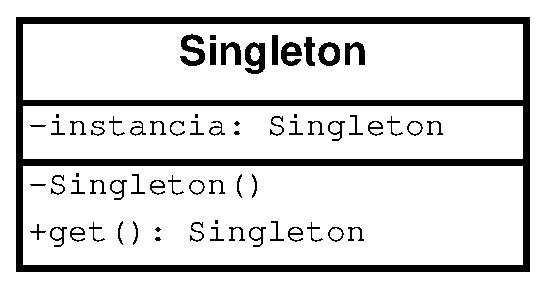
\includegraphics[scale=0.4]{dia-class-singleton}
  \caption{Diagrama UML del patrón Singleton\cite{DesignPatternsLasater}.}
  \label{fig:dia-class-singleton}
\end{figure}

\section{Patrón Estrategia}\label{sec-strategy}
El patrón de diseño Estrategia es un patrón de diseño de comportamiento, es un grupo de algoritmos encapsulados en clases específicas que pueden ser intercambiadas de modo tal que dependiendo del uso específico se selecciona la clase adecuada. El patrón Estrategia expone una clase llamada contexto mediante la cual se tiene acceso a las clases con estrategias específicas que implementan una misma interfaz como se muestra en la Figura \ref{fig:dia-class-strategy} \cite{DesignPatternsLasater, DesignPatterns}.

\begin{figure}[h]
  \centering
  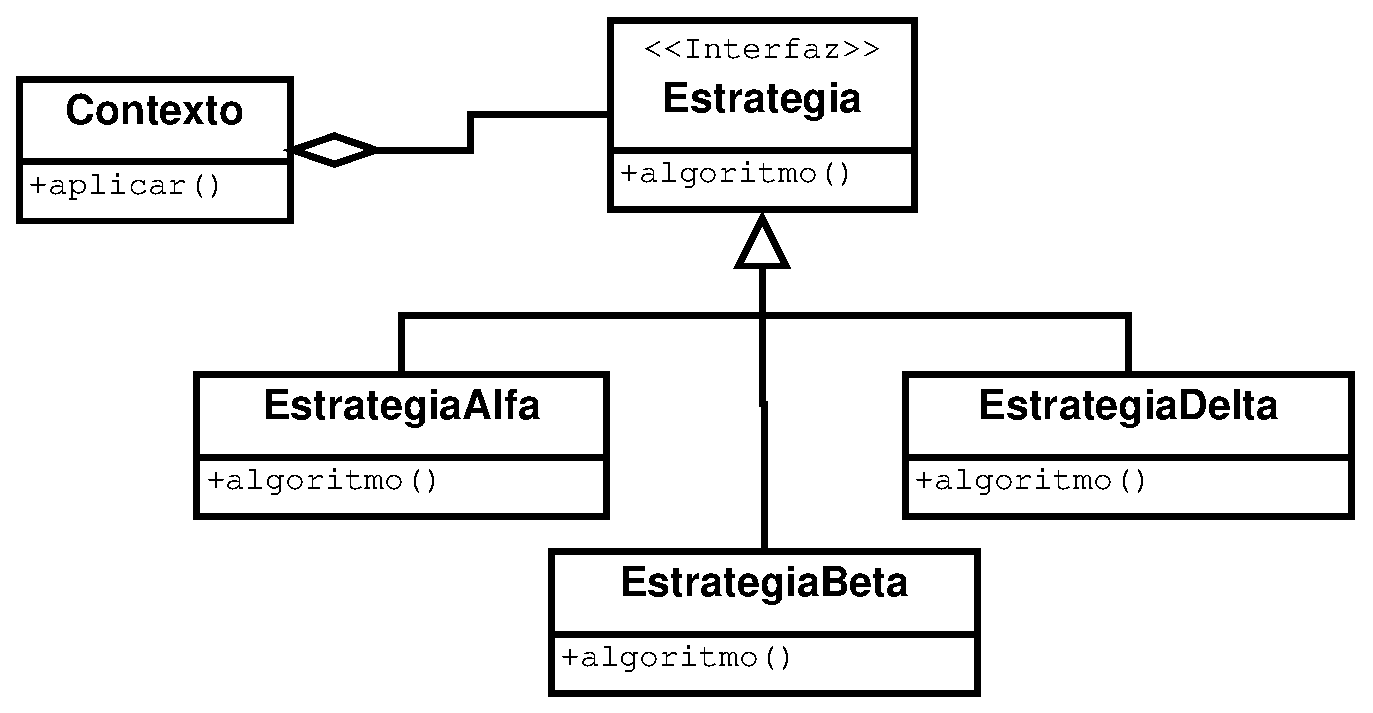
\includegraphics[scale=0.4]{dia-class-strategy}
  \caption{Diagrama UML del patrón Strategy\cite{DesignPatternsLasater}.}
  \label{fig:dia-class-strategy}
\end{figure}

\section{Patrón Decorador}\label{sec-decorator}
El patrón Decorador es utilizado para agregar comportamiento adicional a una clase, tiene cuatro partes principales\cite{DesignPatternsLasater} (ver Figura \ref{fig:dia-class-decorator}):
\begin{enumerate}
  \item Componente: es una clase abstracta que contiene la funcionalidad básica para las clases no decoradas y las decoradas.
  \item Componente concreto: es la implementación de la clase Componente.
  \item Decorador: esta clase es hija de la clase Componente y envuelve una instancias del Componente concreto.
  \item Decorador concreto: es la implementación de la clase que agrega la funcionalidad a la instancia de la clase Componente.
\end{enumerate}

\begin{figure}[h]
  \centering
  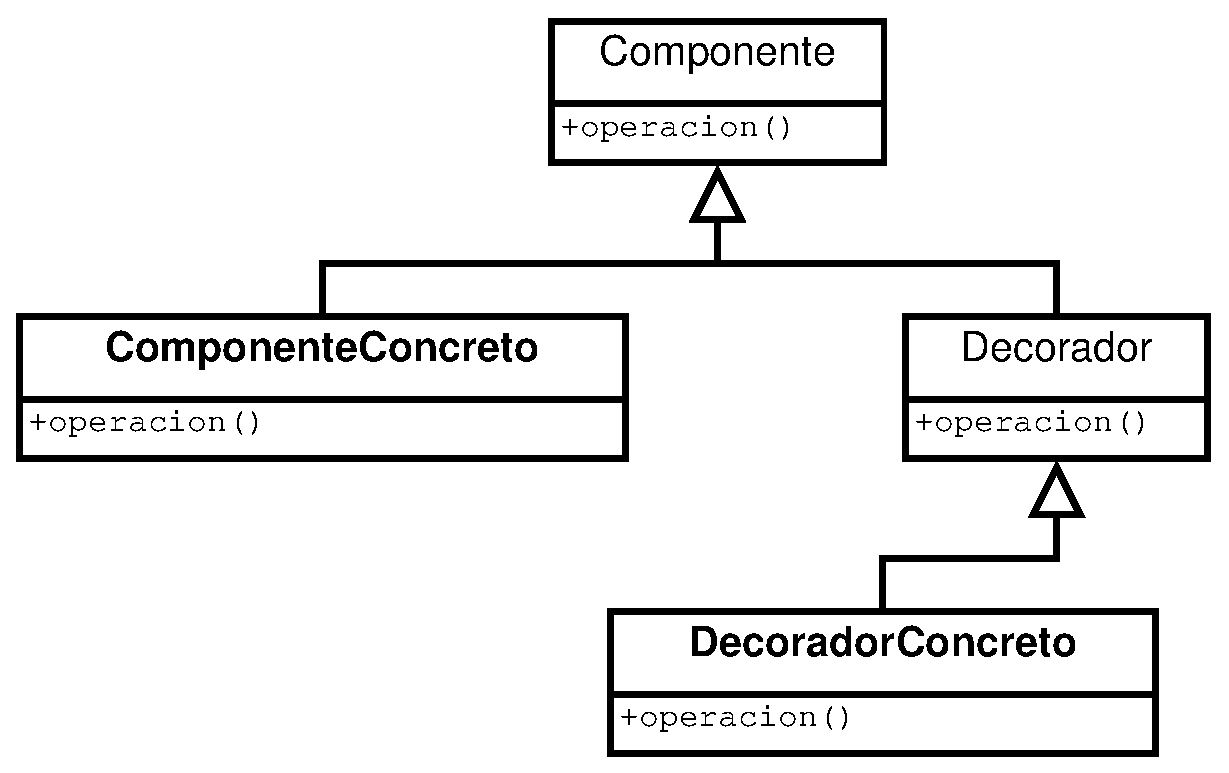
\includegraphics[scale=0.4]{dia-class-decorator}
  \caption{Diagrama UML del patrón Decorador\cite{DesignPatternsLasater}.}
  \label{fig:dia-class-decorator}
\end{figure}

\section{Patrón Proxy}\label{sec-proxy}
El patrón Proxy es una clase que actuá como punto de acceso a otra clase la cual tiene la funcionalidad deseada por algún cliente\cite{DesignPatternsLasater} (ver Figura \ref{fig:dia-class-proxy}):
\begin{enumerate}
  \item Tema: define una interfaz en común para el Tema real y el Proxy.
  \item Tema real: es la clase concreta que representa el Proxy.
  \item Proxy: mantiene referencia a una instancia de la clase Tema real y actúa como punto de acceso a la misma clase.
\end{enumerate}
\begin{figure}[h]
  \centering
  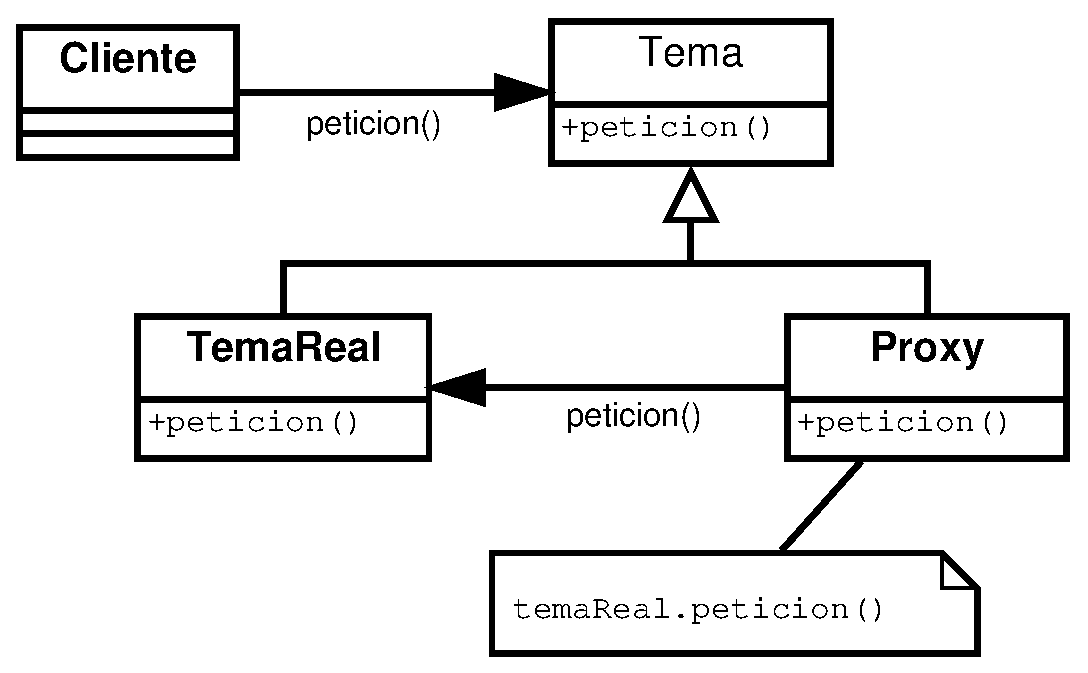
\includegraphics[scale=0.4]{dia-class-proxy}
  \caption{Diagrama UML del patrón Proxy\cite{DesignPatternsLasater}.}
  \label{fig:dia-class-proxy}
\end{figure}

\section{Patrón Objeto de Acceso a Datos}\label{sec-dao}
El patrón Objeto de Acceso a Datos (DAO por sus siglas en inglés) encapsula y abstrae la conexión a una fuente de datos (archivos de texto plano, bases de datos relacionales, bases de datos no relacionales, etc.) y expone operaciones pertinentes al manejo de tales datos\cite{OCPJavaSE7,OCAPJavaSE7}:
\begin{enumerate}
	\item [] \textbf{buscar}: realiza la búsqueda de un único elemento, en caso de no encontrarse tal elemento la respuesta es nula.
	\item [] \textbf{listar}: extrae todos los elementos, el resultado puede utilizar estrategias de paginación.
	\item [] \textbf{insertar}: guarda un nuevo elemento en la fuente de datos.
	\item [] \textbf{actualizar}: actualiza la información de un elemento existente en la fuente de datos.
	\item [] \textbf{borrar}: borra el registro de un elemento en la fuente de datos.
\end{enumerate}


\section{Patrón Modelo-Vista-Controlador}\label{sec-mvc}
Para Sarcar\cite{JavaDesignPatternsExamples} el patrón Modelo Vista Controlador (MVC) es un patrón de arquitectura que consiste de tres grandes componentes: Modelo, Vista y Controlador. El Controlador conduce la comunicación entre la Vista y el Modelo, en la Figura \ref{fig:dia-mvc-simple} se muestra el flujo de comunicación entre los componentes MVC.
\begin{enumerate}
	\item \textbf{Modelo}: tiene la responsabilidad de manejar el acceso a los datos persistentes y la lógica de negocio, usualmente se acompaña del patrón DAO (ver sección \ref{sec-dao}) para el manejo de datos.
	\item \textbf{Vista}: es la capa de presentación, es responsable de mostrar los datos al actor\footnote{Puede ser una persona u otro sistema} que use el sistema.
	\item \textbf{Controlador}: es el intermediario entre la Vista y el Modelo: comunica las peticiones de la vista al modelo y los datos del modelo a la vista.
\end{enumerate}
\begin{figure}[h]
  \centering
  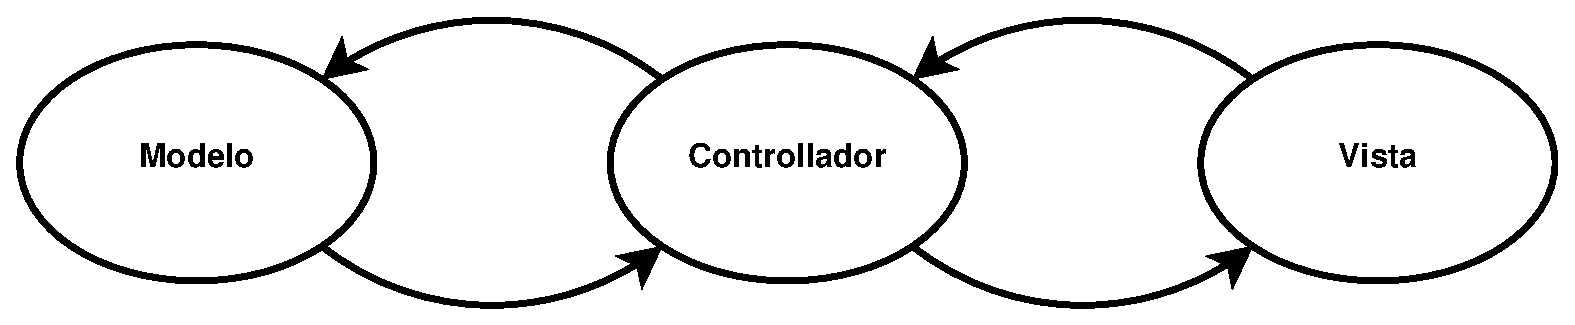
\includegraphics[scale=0.4]{dia-mvc-simple}
  \caption{Diagrama del patrón MVC\cite{JavaDesignPatternsExamples}.}
  \label{fig:dia-mvc-simple}
\end{figure}

%\section{Inversión de control}\label{sec-ioc}
%\textcolor{blue}{Vale por la descripción de inversión de control.}

%\section{Inyección de dependencia}\label{sec-dep-inj}
%\textcolor{blue}{Vale por la descripción de inyección de dependencia.}

\iffalse
%\section{Arquitectura 4+1} Organiza cada decisión en el diseño del sistema en cuatro partes llamadas vistas (ver Figura \ref{fig:dia-arq-4-1}), cada vista se encarga de enfocarse en un aspecto del diseño, estas cuatro vistas son unificadas por una cuarta vista de escenarios o casos de uso\cite{ViewModel4plus1}:
%\begin{itemize}
%	\item \textbf{Vista Lógica}: son las reglas del negocio por las que se rige la operación del usuario final.
%	\item \textbf{Vista de Proceso}: refleja concurrencia y sincronización.
%	\item \textbf{Vista de Física}: describe las relaciones del software con el hardware.
%	\item \textbf{Vista de Desarrollo}: describe la organización estática del software en su ambiente de desarrollo.
%\end{itemize}
%
%\begin{figure}[h]
%\centering
%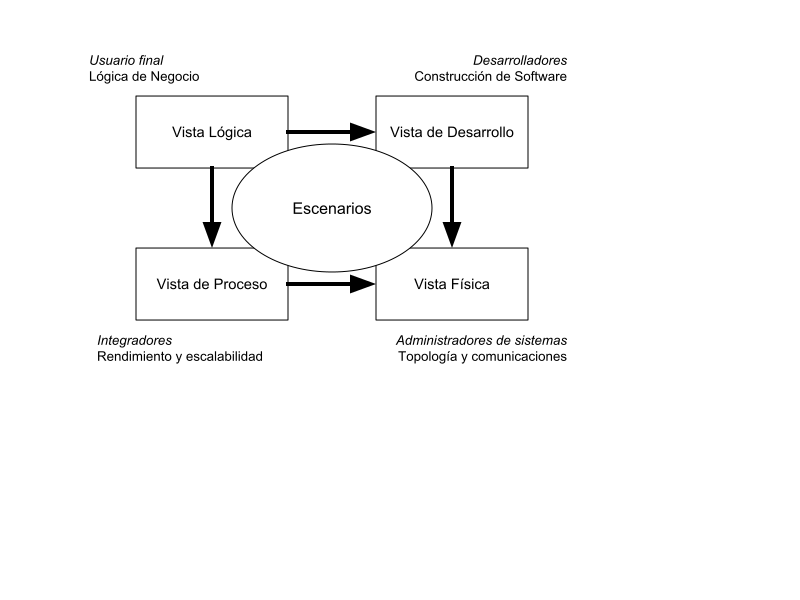
\includegraphics[scale=0.5]{dia-arq-4-1} 
%\caption{Diagrama de arquitectura 4+1.\cite{ViewModel4plus1}}
%\label{fig:dia-arq-4-1}
%\end{figure}
%
%
%\section{Arquitectura Orientada a Servicios}
%Thomas Erl describe la Arquitectura Orientada a Servicios (\textbf{SOA} por sus siglas en inglés) como el modelo arquitectónico del cómputo orientado a servicios\cite{SOAWithRest}, a continuación se muestran las definiciones de Erl sobre los conceptos de Orientación a Servicios:
%\begin{quote}
%La \textbf{Orientación a Servicios} es el paradigma de diseño dedicado para la creación de unidades lógicas de solución que son moldeados individualmente para que puedan ser utilizados colectiva y repetidamente para la realización de objetivos estratégicos y beneficios asociados con el cómputo orientado a servicios.\\
%El \textbf{Cómputo Orientado a Servicios} es engloba distintas plataformas de cómputo distribuido. En sí envuelve su propio paradigma y principios de diseño, catálogos de diseño de patrones, lenguajes, modelo arquitectónico junto con sus conceptos relacionados, tecnologías y marcos de trabajo.\\
%La \textbf{Arquitectura Orientada a Servicios} es un modelo de tecnología arquitectónica para soluciones orientadas a servicios con distintas características en apoyo de realizar orientación a servicios y los objetivos estratégicos asociados con el cómputo orientado a servicios.\cite{SOAWithRest}
%\end{quote}
\fi
%\chapter{Diccionario de Datos}


\section{Tablas}

\paragraph*{sesion} Define una sesión bajo la cual se ejecuta un script de automatización, la sesión puede definir implísitamente un usuario y un rol.
\begin{longtable}{p{4cm}|l|p{8.5cm}}
	\textbf{Columna} &	\textbf{Tipo} &	\textbf{Descripción} \\
	\hline\hline
	{\fontfamily{pcr}\selectfont id}& number & Número identificador \\
	\hline
	{\fontfamily{pcr}\selectfont id{\textunderscore}usuario} & number & Identificador de usuario que creó la sesión \\
	\hline
	{\fontfamily{pcr}\selectfont fecha{\textunderscore}creacion} & datetime & Hora y fecha en que se registró la sesión. Default: CURRENT{\textunderscore}TIMESTAMP \\ 
	\hline
	{\fontfamily{pcr}\selectfont id{\textunderscore}usuario{\textunderscore}fin} & number & Identificador de usuario que finalizó la sesión \\
	\hline
	{\fontfamily{pcr}\selectfont fecha{\textunderscore}fin} & datetime & Hora y fecha en que se finalizó la sesión\\
	\hline
	{\fontfamily{pcr}\selectfont activa} & number & Indicador de actividad en la sesión. Default: 1\\
	\hline
	{\fontfamily{pcr}\selectfont rol} & number & Rol para el cuál fue creada la sesión.\\
	\caption{Tabla sesion.}\label{tab:tab-sesion}
\end{longtable}

\paragraph*{bitacora} Lleva el registro de eventos ocurridos durante la ejecución del script de automatización, el evento puede estar ligado a una sesión.
\begin{longtable}{p{4cm}|l|p{8.5cm}}
	\textbf{Columna} &	\textbf{Tipo} &	\textbf{Descripción} \\
	\hline\hline
	{\fontfamily{pcr}\selectfont id} & number & Número identificador\\
	\hline
	{\fontfamily{pcr}\selectfont id{\textunderscore}sesion} & number & Identificador de sesión desde la cual se hizo el registro.\\
	\hline
	{\fontfamily{pcr}\selectfont fecha} & datetime & Hora y fecha en la que se realizó el registro Default: CURRENT{\textunderscore}TIMESTAMP\\
	\hline
	{\fontfamily{pcr}\selectfont descripcion} & text & Descripción del evento.\\
\caption{Tabla bitacora.}\label{tab:tab-bitacora}
\end{longtable}

\paragraph*{ordenes{\textunderscore}imss} Contiene el registro de las órdenes de reposición del portal SAI que han sido procesadas por el script de automatización.
%\begin{landscape}
\begin{longtable}{p{4cm}|l|p{8.5cm}}
	\textbf{Columna} &	\textbf{Tipo} &	\textbf{Descripción} \\
	\hline\hline
	{\fontfamily{pcr}\selectfont id} & number & Número identificador\\
	\hline
	{\fontfamily{pcr}\selectfont contrato} & text & Cadena alfanumérica con el identificador de contrato\\
	\hline
	{\fontfamily{pcr}\selectfont solicitud} & number & Número de solicitud\\
	\hline
	{\fontfamily{pcr}\selectfont orden} & number & Número de orden de reposición\\
	\hline
	{\fontfamily{pcr}\selectfont fecha{\textunderscore}expedicion} & text & Fecha de expedición\\
	\hline
	{\fontfamily{pcr}\selectfont almacen{\textunderscore}destino} & number & Número identificador del almacén destino\\
	\hline
	{\fontfamily{pcr}\selectfont estatus} & number & Estatus en el proceso de atención Default: 1\\
	\hline
	{\fontfamily{pcr}\selectfont cbb} & number & Clave de Cuadro Básico\\
	\hline
	{\fontfamily{pcr}\selectfont fecha{\textunderscore}vencimiento} & text & Fecha de vencimiento\\
	\hline
	{\fontfamily{pcr}\selectfont cantidad} & number & Cantidad solicitada\\
	\hline
	{\fontfamily{pcr}\selectfont fecha{\textunderscore}insersion} & datetime & Fecha en la que fue registrada la orden en la base de datos. Default: CURRENT{\textunderscore}TIMESTAMP\\
	\hline
	{\fontfamily{pcr}\selectfont fecha{\textunderscore}estatus} & datetime & Fecha en la que se registró el último cambio de estatus Default: CURRENT{\textunderscore}TIMESTAMP\\
	\hline
	{\fontfamily{pcr}\selectfont id{\textunderscore}sesion{\textunderscore} insersion} & number & Identificador de la sesión que realizó el registro en la base de datos\\
	\hline
	{\fontfamily{pcr}\selectfont id{\textunderscore}sesion{\textunderscore}estatus} & number & Identificador de la sesión que realizó el último cambio de estatus\\
	\hline
	{\fontfamily{pcr}\selectfont url{\textunderscore}con} & text & URL de SAI para realizar la contestación\\
	\hline
	{\fontfamily{pcr}\selectfont url{\textunderscore}env} & text & URL de SAI para realizar el envío\\
	\hline
	{\fontfamily{pcr}\selectfont confirmacion} & number & Número de confirmación de envío\\
	\hline
	{\fontfamily{pcr}\selectfont articulo} & text & Artículo según la descripción del campo en la pantalla de finalización de SAI\\
	\hline
	{\fontfamily{pcr}\selectfont unidad} & text & Unidad a la que se refiere la cantidad solicitada según la pantalla de finalización de SAI\\
	\hline
	{\fontfamily{pcr}\selectfont precio} & number & Precio por unidad\\
	\hline
	{\fontfamily{pcr}\selectfont lugar{\textunderscore}entrega} & text & Lugar de entrega\\
	\hline
	{\fontfamily{pcr}\selectfont lote} & text & Identificador del lote\\
	\hline
	{\fontfamily{pcr}\selectfont fecha{\textunderscore}fabricacion} & text & Fecha de fabricación\\
	\hline
	{\fontfamily{pcr}\selectfont fecha{\textunderscore}caducidad} & text & Fecha de caducidad\\
	\hline
	{\fontfamily{pcr}\selectfont marca} & text & La marca del medicamento como se describe en la pantalla de contestación\\
	\hline
	{\fontfamily{pcr}\selectfont procedencia} & text & La procedencia del medicamento como se describe en la pantalla de contestación\\
	\hline
	{\fontfamily{pcr}\selectfont estatus{\textunderscore}sai} & number & Estatus de la orden de reposición en el portal SAI\\
	\hline
	{\fontfamily{pcr}\selectfont estatus{\textunderscore}sap} & number & Estatus de la orden de reposición en el sistema interno de MAYPO\\

	\caption{Tabla ordenes{\textunderscore}imss.}\label{tab:tab-ordenes-imss}
\end{longtable}
%\end{landscape}

\paragraph*{cat{\textunderscore}estatus{\textunderscore}orden} Este catálogo no debe ser alterado, contiene los posibles estatus que pude tomar una orden durante el ciclo de vida de la aplicación.
\begin{longtable}{p{4cm}|l|p{8.5cm}}
	\textbf{Columna} &	\textbf{Tipo} &	\textbf{Descripción} \\
	\hline\hline
	{\fontfamily{pcr}\selectfont id} & number & Número identificador \\
	\hline
	{\fontfamily{pcr}\selectfont nombre} & text & Nombre corto del estatus\\
	\caption{Tabla cat{\textunderscore}estatus{\textunderscore}orden.}\label{tab:tab-cat-estatus-orden}
\end{longtable}

\paragraph*{cat{\textunderscore}estatus{\textunderscore}sai} Este catálogo contiene los estados definidos por el portal SAI para una orden de reposición.
\begin{longtable}{p{4cm}|l|p{8.5cm}}
	\textbf{Columna} &	\textbf{Tipo} &	\textbf{Descripción} \\
	\hline\hline	
	{\fontfamily{pcr}\selectfont id} & number & Número identificador \\
	\hline
	{\fontfamily{pcr}\selectfont nombre} & text & Nombre corto del estatus\\
	\caption{Tabla cat{\textunderscore}estatus{\textunderscore}sai.}\label{tab:tab-cat-estatus-sai}
\end{longtable}

\paragraph*{cat{\textunderscore}clientes} Este catálogo refleja el contenido necesario para la generación del layout de SAP ubicado en la hoja CLIENTES del archivo LICITACION  CARGA IMSS 2014.xlsx.
\begin{longtable}{p{4cm}|l|p{8.5cm}}
	\textbf{Columna} &	\textbf{Tipo} &	\textbf{Descripción} \\
	\hline\hline	
	{\fontfamily{pcr}\selectfont lugar{\textunderscore}entrega} & number & Columna A, LUGAR DE ENTREGA\\
	\hline
	{\fontfamily{pcr}\selectfont factura} & number & Columna B, FACTURA\\
	\hline
	{\fontfamily{pcr}\selectfont destino}  & number & Columna C, DESTINO\\
	\hline
	{\fontfamily{pcr}\selectfont consignado{\textunderscore} controlado}  & number & Columna D, CONSIGNADO CONTROLADO\\
	\hline
	{\fontfamily{pcr}\selectfont almacen} & text & Columna E, ALMACEN \\
	\hline
	{\fontfamily{pcr}\selectfont entrega} & text & Columna F, ENTREGA\\
	\caption{Tabla cat{\textunderscore}clientes.}\label{tab:tab-cat-clientes}
\end{longtable}

\paragraph*{cat{\textunderscore}contratos} Este catálogo refleja el contenido necesario para la generación del layout de SAP ubicado en la hoja CONTRATOS del archivo LICITACION  CARGA IMSS 2014.xlsx.
\begin{longtable}{p{4cm}|l|p{8.5cm}}
	\textbf{Columna} &	\textbf{Tipo} &	\textbf{Descripción} \\
	\hline\hline	
	{\fontfamily{pcr}\selectfont pedido} & text & Columna B, No PEDIDO\\
	\hline
	{\fontfamily{pcr}\selectfont documento{\textunderscore} comercial} & number & Columna C, DOCUMENTO  COMERCIAL\\
	\hline
	{\fontfamily{pcr}\selectfont cbb} & number & Columna F, CCB\\
	\hline
	{\fontfamily{pcr}\selectfont material} & number & Columna G, MATERIAL\\
	\hline
	{\fontfamily{pcr}\selectfont tipo} & text & Columna I, TIPO\\
	\hline
	{\fontfamily{pcr}\selectfont etiqueta} & text & Columna Q, ETIQUETA\\
	\hline
	{\fontfamily{pcr}\selectfont fianza} & number & Columna U, FIANZA\\
	\caption{Tabla cat{\textunderscore}contratos.}\label{tab:tab-cat-contratos}
\end{longtable}


\section{Vistas}
\paragraph*{matriz{\textunderscore}imss} Esta vista refleja el contenido necesario para la generación del layout de SAP ubicado en la hoja MATRIZ del archivo LICITACION  CARGA IMSS 2014.xlsx.
\begin{longtable}{p{4cm}|l|p{8.5cm}}
	\textbf{Columna} &	\textbf{Tipo} &	\textbf{Descripción} \\
	\hline\hline
	{\fontfamily{pcr}\selectfont documento{\textunderscore} comercial} & number & El máximo de la columna documento{\textunderscore}comercial de los renglones del catálogo de contratos cuyos contrato y CCB sean iguales sean iguales a los de la orden de reposición.\\
	\hline
	{\fontfamily{pcr}\selectfont fianza} & number & El máximo de la columna fianza de los renglones del catálogo de contratos cuyos contrato y CCB sean iguales sean iguales a los de la orden de reposición.\\
	\hline
	{\fontfamily{pcr}\selectfont solicitud} & number & Columna solicitud de la orden.\\
	\hline
	{\fontfamily{pcr}\selectfont fecha{\textunderscore}expedicion} & text & Columna fecha{\textunderscore}expedicion de la orden.\\
	\hline
	{\fontfamily{pcr}\selectfont orden} & number & Columna orden de la orden de reposición.\\
	\hline
	{\fontfamily{pcr}\selectfont factura} & number & El máximo de la columna factura de los renglones del catálogo de clientes cuyo almacén destino de la orden de reposición sea igual al lugar de entrega del catálogo.\\
	\hline
	{\fontfamily{pcr}\selectfont cte{\textunderscore}destino} & number & Sí el tipo del contrato de la orden de reposición es CONTROLADO, entonces se debe tomar el máximo valor de la columna consigando{\textunderscore}controlado del catálogo de clientes cuyo almacén destino de la orden de reposición sea igual al lugar de entrega del catálogo. En caso contrario se debe tomar el máximo de la columna destino con los mismos criterios del caso anterior.\\
	\hline
	{\fontfamily{pcr}\selectfont entrega} & text & El máximo de la columna entrega de los renglones del catálogo de clientes cuyo almacén destino de la orden de reposición sea igual al lugar de entrega del catálogo.\\
	\hline
	{\fontfamily{pcr}\selectfont material} & number & El máximo de la columna material de los renglones del catálogo de contratos cuyos contrato y CCB sean iguales sean iguales a los de la orden de reposición.\\
	\hline
	{\fontfamily{pcr}\selectfont instrucciones{\textunderscore} etiquetado} & text & Columna U, INSTRUCCIONES DE ETIQUETADO  (archivo Excel)
El máximo de la concatenación de las columnas etiqueta y cbb (separadas por un espacio) de los renglones del catálogo de contratos cuyos contrato y CCB sean iguales a los de la orden de reposición.\\
	\hline
	{\fontfamily{pcr}\selectfont cantidad} & number & Cantidad solicitada de la orden de reposición\\
	\hline
	{\fontfamily{pcr}\selectfont fecha{\textunderscore}vencimiento} & text & Fecha de vencimiento de la orden de reposición\\
	\hline
	{\fontfamily{pcr}\selectfont sesion} & number & Sesión con la cual fue finalizada la orden de reposición, esta columna no está contenida en el archivo de Excel. Identificador de la sesión que realizó el último cambio de estatus.\\
	\caption{Tabla matriz{\textunderscore}imss.}\label{tab:tab-matriz-imss}
\end{longtable}

\paragraph*{layout{\textunderscore}imss{\textunderscore}sap} Esta vista refleja el contenido de la hoja Formato de carga SAP del archivo CARGA MASIVA IMSS HECTOR.xlsm después de haber aplicado la macro que contiene sobre el archivo LICITACION  CARGA IMSS 2014.xlsx.
\begin{longtable}{p{4cm}|l|p{8.5cm}}
	\textbf{Columna} &	\textbf{Tipo} &	\textbf{Descripción} \\
	\hline\hline
	{\fontfamily{pcr}\selectfont documento{\textunderscore} comercial} & number & Columna A, DSADAS Columna documento{\textunderscore}comercial de vista matriz{\textunderscore}imss\\
	\hline
	{\fontfamily{pcr}\selectfont solicitante} & number & Columna B, Solicitante Valor constante 100002\\
	\hline
	{\fontfamily{pcr}\selectfont solicitud} & number & Columna C, SOLICITUD Columna solicitud de vista matriz{\textunderscore}imss\\
	\hline
	{\fontfamily{pcr}\selectfont fecha{\textunderscore}expedicion} & text & Columna D, FECHA DE EXPEDICIÓN Columna fecha{\textunderscore}expedicion de vista matriz{\textunderscore}imss\\
	\hline
	{\fontfamily{pcr}\selectfont orden} & number & Columna E, ORDEN REPOSICIÓN Columna orden de vista matriz{\textunderscore}imss\\
	\hline
	{\fontfamily{pcr}\selectfont factura} & number & Columna F, CTE FACTURA Columna factura de vista matriz{\textunderscore}imss\\
	\hline
	{\fontfamily{pcr}\selectfont cte{\textunderscore}destino} & number & Columna G, CTE DESTINO Columna cte{\textunderscore}destino de vista matriz{\textunderscore}imss\\
	\hline
	{\fontfamily{pcr}\selectfont material} & number & Columna H, MATERIAL SAP Columna material de vista matriz{\textunderscore}imss\\
	\hline
	{\fontfamily{pcr}\selectfont instrucciones{\textunderscore} etiquetado} & number & Columna I, INTRUCCIONES DE ETIQUETADO Columna instrucciones{\textunderscore}etiquetado de vista matriz{\textunderscore}imss\\
	\hline
	{\fontfamily{pcr}\selectfont cantidad} & number & Columna J, CANTIDAD SOLICITADA Columna cantidad de vista matriz{\textunderscore}imss\\
	\hline
	{\fontfamily{pcr}\selectfont fecha{\textunderscore}limite} & text & Columna K, FECHA LÍMITE Columna fecha{\textunderscore}vencimiento de vista matriz{\textunderscore}imss\\
	\hline
	{\fontfamily{pcr}\selectfont fianza} & number & Columna L, Número de fianza Columna fianza de vista matriz{\textunderscore}imss\\
	\hline
	{\fontfamily{pcr}\selectfont fecha{\textunderscore}preferente} & text & Columna M, Fecha preferente de entrega Columna fecha{\textunderscore}vencimiento de vista matriz{\textunderscore}imss\\
	\hline
	{\fontfamily{pcr}\selectfont entrega} & text & Columna N, Instrucciones para distribución Columna entrega de vista matriz{\textunderscore}imss\\
	\hline
	{\fontfamily{pcr}\selectfont sesion} & number & Sesión con la cual fue finalizada la orden de reposición, esta columna no está contenida en el archivo de Excel.\\
	\caption{Tabla layout{\textunderscore}imss{\textunderscore}sap.}\label{tab:tab-layout-imss-sap}
\end{longtable}
%\chapter{Detalle de las opreciones de las interfaces del componentes}
\subsubsection{Lógica de Automatización}
La función de este componente es de ejecutar las reglas de negocio necesarias para en los flujos de los procesos de automatización, ofrece las interfaces de repuesta y verificación.
\paragraph{Interfaz Respuesta\\}
Provee el acceso a las reglas de negocio del proceso de respuesta de órdenes de reposición (ver caso de uso \ref{cu-contestar}).\\
Esta interfaz expone las siguientes operaciones:\\
\textbf{guardar-orden-nueva}:\quad realiza la lógica de negocio correspondiente a guardar la información de una orden de reposición que se muestra en el listado de órdenes del Sistema de Abastecimiento.
\vspace{3mm}\\
%\noindent
	\begin{tabular}{|p{\dimexpr.2\textwidth}|p{\dimexpr.8\textwidth-4\tabcolsep}|}
		\hline
		\textbf{Identificador}	& \textbf{guardar-orden-nueva}\\
		\hline
		\hline
		\textbf{Descripción}	& Guarda un listado de nuevas órdenes de reposición.\\
		\hline
		\textbf{Parámetros}		& \textbullet\, Listado de mapas, cada mapa contiene los datos de una orden de reposición.\\
		\hline
		\textbf{Salida}			& No ofrece resultado.\\
		\hline
	\end{tabular}
	\vspace{3mm}\\
\textbf{guardar-orden-nueva}:\quad La operación  realiza la lógica de negocio correspondiente a guardar la información de una orden de reposición que se muestra en el listado de órdenes del Sistema de Abastecimiento.\\
	\begin{tabular}{|p{\dimexpr.2\textwidth}|p{\dimexpr.8\textwidth-4\tabcolsep}|}
		\hline
		\textbf{Identificador}	& \textbf{obtener-orden-contestar}\\
		\hline
		\hline
		\textbf{Descripción}	& Da la siguiente orden de reposición para contestar.\\
		\hline
		\textbf{Parámetros}		& \textbullet\, No recibe parámetros.\\
		\hline
		\textbf{Salida}			& Mapa con la información de la orden de reposición.\\
		\hline
	\end{tabular}
	\begin{longtable}{|p{\dimexpr.2\textwidth}|p{\dimexpr.8\textwidth-4\tabcolsep}|}
		\hline
		\textbf{Identificador}	& \textbf{obtener-datos-respuesta}\\
		\hline
		\hline
		\textbf{Descripción}	& Da los datos necesarios para llenar los formularios para contestar una orden de reposición en el Sistema de Abastecimiento.\\
		\hline
		\textbf{Parámetros}		& \textbullet\, Mapa con los datos de la orden para contestar.\\
		\hline
		\textbf{Salida}			& Mapa con la información para llenar los formularios para contestar la orden de reposición.\\
		\hline
	\end{longtable}
	\begin{longtable}{|p{\dimexpr.2\textwidth}|p{\dimexpr.8\textwidth-4\tabcolsep}|}
		\hline
		\textbf{Identificador}	& \textbf{actualizar-orden-contestada}\\
		\hline
		\hline
		\textbf{Descripción}	& Actualiza los datos guardados de la orden de reposición con los datos de la respuesta en el  Sistema de Abastecimiento. Utiliza el componente de persistencia para actualizar los datos.\\
		\hline
		\multirow{2}{*}{\textbf{Parámetros}}	& \textbullet\, Número de orden.\\
												& \textbullet\, Mapa con los datos para guardar.\\
		\hline
		\textbf{Salida}			& No ofrece resultado.\\
		\hline
	\end{longtable}
	\begin{longtable}{|p{\dimexpr.2\textwidth}|p{\dimexpr.8\textwidth-4\tabcolsep}|}
		\hline
		\textbf{Identificador}	& \textbf{obtener-orden-enviar}\\
		\hline
		\hline
		\textbf{Descripción}	& Da la siguiente orden de reposición para enviar.\\
		\hline
		\textbf{Parámetros}		& \textbullet\, No recibe parámetros.\\
		\hline
		\textbf{Salida}			& Mapa con la información de la orden de reposición.\\
		\hline
	\end{longtable}
	\begin{longtable}{|p{\dimexpr.2\textwidth}|p{\dimexpr.8\textwidth-4\tabcolsep}|}
		\hline
		\textbf{Identificador}	& \textbf{guardar-orden-enviada}\\
		\hline
		\hline
		\textbf{Descripción}	& Actualiza los datos guardados de la orden de reposición con los datos de la pantalla de envío del Sistema de Abastecimiento. Utiliza el componente de persistencia para actualizar los datos.\\
		\hline
		\multirow{2}{*}{\textbf{Parámetros}}	& \textbullet\, Número de orden.\\
												& \textbullet\, Mapa con los datos para guardar.\\
		\hline
		\textbf{Salida}			& No ofrece resultado.\\
		\hline
	\end{longtable}
	\begin{longtable}{|p{\dimexpr.2\textwidth}|p{\dimexpr.8\textwidth-4\tabcolsep}|}
		\hline
		\textbf{Identificador}	& \textbf{obtener-acuse-envio}\\
		\hline
		\hline
		\textbf{Descripción}	& Solicita la generación de el acuse de envío al componente de reportes y almacena el documento el componente de Sistema de Archivos.\\
		\hline
		\textbf{Parámetros}		& \textbullet\, Número de orden.\\
		\hline
		\textbf{Salida}			& No ofrece resultado.\\
		\hline
	\end{longtable}
	\vspace{5mm}

\paragraph{Verificación\\}
Provee el acceso a las reglas de negocio del proceso de verificación de órdenes de reposición canceladas.

	\begin{longtable}{|p{\dimexpr.2\textwidth}|p{\dimexpr.8\textwidth-4\tabcolsep}|}
		\hline
		\textbf{Identificador}	& \textbf{obtener-rango-verificar}\\
		\hline
		\hline
		\textbf{Descripción}	& Obtiene el rango de fechas para ingresar en el formulario de búsqueda del Sistema de Abastecimiento. El número de días que comprende el rango se obtiene utilizando el componente de Sistema de Archivos.\\
		\hline
		\textbf{Parámetros}		& \textbullet\, No tiene parámetros.\\
		\hline
		\textbf{Salida}			& El número de días para el rango de búsqueda.\\
		\hline
	\end{longtable}

	\begin{longtable}{|p{\dimexpr.2\textwidth}|p{\dimexpr.8\textwidth-4\tabcolsep}|}
		\hline
		\textbf{Identificador}	& \textbf{actualizar-estado-sa}\\
		\hline
		\hline
		\textbf{Descripción}	& Actualiza el EstadoSA de las órdenes de reposición recibidas a \textbf{Cancelada}. Utiliza el componente de persistencia para la actualización de datos.\\
		\hline
		\textbf{Parámetros}		& \textbullet\, Listado con los números de las órdenes de reposición canceladas.\\
		\hline
		\textbf{Salida}			& El número de órdenes de reposición actualizadas.\\
		\hline
	\end{longtable}

\subsubsection{Persistencia}
El componente de persistencia está basado en el patrón de diseño \textit{DAO} (ver apéndice \ref{sec-dao}) para controlar el acceso a la base de datos\footnote{En adelante se utilizará \textbf{DAO} para hacer referencia al patrón y la instancia (objeto) del patrón.}.\\
El componente de persistencia de el proyecto AutoSA presenta las siguientes interfaces de búsqueda y almacenamiento:
\paragraph{Almacenamiento\\}
Conjunto de operaciones diseñadas para responder a las necesidades de almacenamiento en los flujos para responder y verificar órdenes de reposición\footnote{Ver casos de uso \ref{cu-contestar}, \ref{cu-guardar-nueva}, \ref{cu-responder-orden}, \ref{cu-enviar-orden} y \ref{cu-actualizar-estatus-sa}.}:

	\begin{longtable}{|p{\dimexpr.2\textwidth}|p{\dimexpr.8\textwidth-4\tabcolsep}|}
		\hline
		\textbf{Identificador}	& \textbf{guardar-nueva} \\
		\hline
		\hline
		\textbf{Descripción}	& Inserta una nueva orden de reposición en la base de datos.\\
		\hline
		\textbf{Parámetros} 	& \textbullet\, Mapa con los datos de la orden de reposición.\\
		\hline
		\textbf{Salida}			& No ofrece resultado.\\
		\hline
	\end{longtable}

	\begin{longtable}{|p{\dimexpr.2\textwidth}|p{\dimexpr.8\textwidth-4\tabcolsep}|}
		\hline
		\textbf{Identificador}	& \textbf{cambiar-estado} \\
		\hline
		\hline
		\textbf{Descripción}	& Cambia el estado de atención de una orden de reposición. \\
		\hline
		\multirow{2}{*}{\textbf{Parámetros}}	& \textbullet\, Número de orden de reposición.\\
												& \textbullet\, Estado.\\
		\hline
		\textbf{Salida}			& No ofrece resultado.\\
		\hline
	\end{longtable}

	\begin{longtable}{|p{\dimexpr.2\textwidth}|p{\dimexpr.8\textwidth-4\tabcolsep}|}
		\hline
		\textbf{Identificador}	& \textbf{guardar-respuesta}\\
		\hline
		\hline
		\textbf{Descripción}	& Guarda los datos de los formularios de la pantalla de respuesta de las órdenes de reposición.\\
		\hline
		\multirow{2}{*}{\textbf{Parámetros}}	& \textbullet\, Número de orden de reposición.\\
												& \textbullet\, Mapa con los datos de los formularios.\\
		\hline
		\textbf{Salida}			& No ofrece resultado.\\
		\hline
	\end{longtable}

	\begin{longtable}{|p{\dimexpr.2\textwidth}|p{\dimexpr.8\textwidth-4\tabcolsep}|}
		\hline
		\textbf{Identificador}	& \textbf{guardar-folio-acuse}\\
		\hline
		\hline
		\textbf{Descripción}	& Guarda el folio de acuse de envío de la orden de reposición.\\
		\hline
		\multirow{2}{*}{\textbf{Parámetros}} 	& \textbullet\, Número de orden de reposición.\\
												& \textbullet\, Folio de acuse de envío.\\
		\hline
		\textbf{Salida}			& No ofrece resultado.\\
		\hline
	\end{longtable}

	\begin{longtable}{|p{\dimexpr.2\textwidth}|p{\dimexpr.8\textwidth-4\tabcolsep}|}
		\hline
		\textbf{Identificador}	& \textbf{actualizar-estado-sa}\\
		\hline
		\hline
		\textbf{Descripción}	& Actualiza el estado de atención en el Sistema de Abastecimiento a \textbf{cancelada} de las órdenes de reposición recibidas.\\
		\hline
		\textbf{Parámetros} 	& \textbullet\, Lista con los números de las órdenes de reposición.\\
		\hline
		\textbf{Salida}			& El número de órdenes de reposición actualizadas.\\
		\hline
	\end{longtable}

	\begin{longtable}{|p{\dimexpr.2\textwidth}|p{\dimexpr.8\textwidth-4\tabcolsep}|}
		\hline
		\textbf{Identificador}	& \textbf{registrar-evento}\\
		\hline
		\hline
		\textbf{Descripción}	& Registra en la base de datos un evento que ocurre durante los procesos automatizados, el evento puede ser de carácter informativo o de error.\\
		\hline
		\multirow{2}{*}{\textbf{Parámetros}}	& \textbullet\, Tipo de evento.\\
												& \textbullet\, Mapa con la descripción del evento.\\
		\hline
		\textbf{Salida}			& No ofrece resultado.\\
		\hline
	\end{longtable}

\paragraph{Lectura\\}
Conjunto de operaciones diseñadas para las necesidades de lectura de órdenes de reposición en los flujos para responder y verificar órdenes de reposición\footnote{Ver casos de uso \ref{cu-contestar}, \ref{cu-enviar-orden} y \ref{cu-generar-acuse}.}:

	\begin{longtable}{|p{\dimexpr.2\textwidth}|p{\dimexpr.8\textwidth-4\tabcolsep}|}
		\hline
		\textbf{Identificador}	& \textbf{siguiente-orden-contestar}\\
		\hline
		\hline
		\textbf{Descripción}	& Entrega un mapa con los datos de la primera orden de reposición encontrada con estado \textbf{Nueva}.\\
		\hline
		\textbf{Parámetros} 	& \textbullet\, No tiene parámetros.\\
		\hline
		\textbf{Salida}			& Un mapa con los datos de la primera orden de reposición encontrada con estado \textbf{Nueva}. En caso de no existir tal orden regresa un mapa vacío.\\
		\hline
	\end{longtable}

	\begin{longtable}{|p{\dimexpr.2\textwidth}|p{\dimexpr.8\textwidth-4\tabcolsep}|}
		\hline
		\textbf{Identificador}	& \textbf{siguiente-orden-enviar}\\
		\hline
		\hline
		\textbf{Descripción}	& Entrega un mapa con los datos de la primera orden de reposición encontrada con estado \textbf{Contestada}.\\
		\hline
		\textbf{Parámetros} 	& \textbullet\, No tiene parámetros.\\
		\hline
		\textbf{Salida}			& Un mapa con los datos de la primera orden de reposición encontrada con estado \textbf{Contestada}. En caso de no existir tal orden regresa un mapa vacío.\\
		\hline
	\end{longtable}

	\begin{longtable}{|p{\dimexpr.2\textwidth}|p{\dimexpr.8\textwidth-4\tabcolsep}|}
		\hline
		\textbf{Identificador}	& \textbf{obtener-datos-acuse}\\
		\hline
		\hline
		\textbf{Descripción}	& Obtiene los datos de una orden de reposición necesarios para generar el documento de acuse de envío.\\
		\hline
		\textbf{Parámetros}		& \textbullet\, Número de orden de reposición.\\
		\hline
		\textbf{Salida}			& Un mapa con los datos de la orden de reposición. En caso de no existir tal orden regresa un mapa vacío.\\
		\hline
	\end{longtable}

\paragraph{Administración\\}
Son las operaciones que permiten modificar datos específicos de las órdenes de reposición contenidas en la base de datos, también ofrece la actualización masiva de catálogos\footnote{Ver casos de uso \ref{cu-entrar-web}, \ref{cu-generar-reporte}, \ref{cu-actualizar-catalogo}, \ref{cu-buscar}, \ref{cu-visualizar} y \ref{cu-editar}.}).

	\begin{longtable}{|p{\dimexpr.2\textwidth}|p{\dimexpr.8\textwidth-4\tabcolsep}|}
		\hline
		\textbf{Identificador}	& \textbf{buscar-credenciales}\\
		\hline
		\hline
		\textbf{Descripción}	& Busca las credenciales del usuario.\\
		\hline
		\textbf{Parámetros}		& \textbullet\, Identificador de usuario.\\
		\hline
		\textbf{Salida}			& Un mapa con las credenciales del usuario.\\
		\hline
	\end{longtable}

	\begin{longtable}{|p{\dimexpr.2\textwidth}|p{\dimexpr.8\textwidth-4\tabcolsep}|}
		\hline
		\textbf{Identificador}	& \textbf{extraer-reporte}\\
		\hline
		\hline
		\textbf{Descripción}	& Ejecuta la búsqueda necesaria para extraer los datos del reporte indicado.\\
		\hline
		\multirow{2}{*}{\textbf{Parámetros}}	& \textbullet\, Tipo de reporte.\\
												& \textbullet\, Mapa con los parámetros del filtro de búsqueda.\\
		\hline
		\textbf{Salida}			& Un listado con los datos del reporte.\\
		\hline
	\end{longtable}

	\begin{longtable}{|p{\dimexpr.2\textwidth}|p{\dimexpr.8\textwidth-4\tabcolsep}|}
		\hline
		\textbf{Identificador}	& \textbf{actualizar-catalogo}\\
		\hline
		\hline
		\textbf{Descripción}	& Actualiza la información del catálogo indicado.\\
		\hline
		\multirow{2}{*}{\textbf{Parámetros}}	& \textbullet\, Identificador del catálogo.\\
												& \textbullet\, Listado con los datos del catálogo.\\
		\hline
		\textbf{Salida}			& El número de los registros insertados en el catálogo.\\
		\hline
	\end{longtable}

	\begin{longtable}{|p{\dimexpr.2\textwidth}|p{\dimexpr.8\textwidth-4\tabcolsep}|}
		\hline
		\textbf{Identificador}	& \textbf{buscar-ordenes}\\
		\hline
		\hline
		\textbf{Descripción}	& Busca órdenes de reposición que cumplan con el filtro de búsqueda indicado.\\
		\hline
		\textbf{Parámetros}		& \textbullet\, Mapa con el filtro de búsqueda.\\
		\hline
		\textbf{Salida}			& Un listado con las órdenes de reposición encontradas.\\
		\hline
	\end{longtable}

	\begin{longtable}{|p{\dimexpr.2\textwidth}|p{\dimexpr.8\textwidth-4\tabcolsep}|}
		\hline
		\textbf{Identificador}	& \textbf{buscar-orden}\\
		\hline
		\hline
		\textbf{Descripción}	& Busca una orden de reposición por el número de orden.\\
		\hline
		\textbf{Parámetros}		& \textbullet\, Número de orden de reposición.\\
		\hline
		\textbf{Salida}			& La orden de reposición encontrada. En caso de no encontrar la orden se regresa un identificador vacío.\\
		\hline
	\end{longtable}

	\begin{longtable}{|p{\dimexpr.2\textwidth}|p{\dimexpr.8\textwidth-4\tabcolsep}|}
		\hline
		\textbf{Identificador}	& \textbf{actualizar-orden}\\
		\hline
		\hline
		\textbf{Descripción}	& Actualiza los datos de orden de reposición.\\
		\hline
		\multirow{2}{*}{\textbf{Parámetros}}	& \textbullet\, Número de orden.\\
												& \textbullet\, Mapa con los datos actualizados.\\
		\hline
		\textbf{Excepciones}	& Error si la orden de reposición no se encuentra registrada en la base de datos.\\
		\hline
	\end{longtable}

\subsubsection{Sistema de Archivos}
El componente Sistema de Archivos es el único que se comunica con el sistema de archivos del sistema operativo\footnote{En este documento se utilizará de forma indistinta el término Sistema de archivos para referirse tanto al componente del sistema AutoSA como al propio del sistema operativo.}, tiene la función de realizar la lectura de archivos de configuración, el almacenamiento de los acuses de envío  y los reportes de las órdenes de reposición.\\
Este componente también está diseñado siguiendo el patrón DAO\footnote{Ver apéndice \ref{sec-dao}.}.
\paragraph{Configuración\\}
Da la configuración contenida en archivos de propiedades contenidas en el mismo sistema de archivos.

	\begin{longtable}{|p{\dimexpr.2\textwidth}|p{\dimexpr.8\textwidth-4\tabcolsep}|}
		\hline
		\textbf{Identificador}	& \textbf{obtener-propiedad}\\
		\hline
		\hline
		\textbf{Descripción}	& Obtiene una propiedad de los archivos de configuración.\\
		\hline
		\textbf{Parámetros}		& \textbullet\, Identificador de la propiedad.\\
		\hline
		\textbf{Salida}			& El valor de la propiedad. Si no existe la propiedad regresa la cadena vacía.\\
		\hline
	\end{longtable}

\paragraph{Almacenamiento\\}
Almacena archivos (reportes y acuses de envío) en el sistema de archivos.

	\begin{longtable}{|p{\dimexpr.2\textwidth}|p{\dimexpr.8\textwidth-4\tabcolsep}|}
		\hline
		\textbf{Identificador}	& \textbf{guardar-archivo}\\
		\hline
		\hline
		\textbf{Descripción}	& Guarda un archivo en el sistema de archivos.\\
		\hline
		\multirow{2}{*}{\textbf{Parámetros}}	& \textbullet\, Archivo.\\
												& \textbullet\, Ruta del archivo.\\
		\hline
		\textbf{Salida}			& No ofrece resultado.\\
		\hline
	\end{longtable}

\subsubsection{Generador de Reportes}
El Generador de Reportes, como su nombre lo indica, tiene la función de generar documentos y reportes con los datos de las órdenes de reposición almacenados en la base de datos. 
\paragraph{Acuse\\} Genera el documento con el acuse de envío.

	\begin{longtable}{|p{\dimexpr.2\textwidth}|p{\dimexpr.8\textwidth-4\tabcolsep}|}
		\hline
		\textbf{Identificador}	& \textbf{generar-acuse-envio}\\
		\hline
		\hline
		\textbf{Descripción}	& Genera el acuse de envío para la orden de reposición especificada. Utiliza el componente de persistencia para obtener los datos de la orden.\\
		\hline
		\textbf{Parámetros}		& \textbullet\, Número de la orden de reposición.\\
		\hline
		\textbf{Salida}			& La ruta en el sistema de archivos donde ha sido depositado el acuse de envío.\\
		\hline
	\end{longtable}

\paragraph{Generación\\} Genera reportes con los datos de las órdenes de reposición almacenados en la base de datos.

	\begin{longtable}{|p{\dimexpr.2\textwidth}|p{\dimexpr.8\textwidth-4\tabcolsep}|}
		\hline
		\textbf{Identificador}	& \textbf{generar-reporte-ordenes}\\
		\hline
		\hline
		\textbf{Descripción}	& Genera el reporte del tipo indicado, usando el rango de fechas establecido.\\
		\hline
		\multirow{3}{*}{\textbf{Parámetros}}	& \textbullet\, Tipo de reporte.\\
												& \textbullet\, Fecha inicial.\\
												& \textbullet\, Fecha final.\\
		\hline
		\textbf{Salida}			& La ruta en el sistema de archivos donde ha sido depositado el reporte generado.\\
		\hline
	\end{longtable}
%\newacronym{api}{API}{Application Programming Interface}
\newacronym{css}{CSS}{Cascading Style Sheet}
\newacronym{csv}{CSV}{Comma Separated Values}
\newacronym{html}{HTML}{Hypertext Markup Language}
\newacronym{jdbc}{JDBC}{Java Data Base Controller}
\newacronym{jdk}{JDK}{Java Development Kit}
\newacronym{pdf}{PDF}{Portable Document Format}
\newacronym{rest}{REST}{Representational State Transfer}
\newacronym{restful}{RESTFUL}{lo mismo que REST, pero al ful}
\newacronym{soa}{SOA}{Service Oriented Architecture}
\newacronym{url}{URL}{Universal Resource Locator}
\newacronym{xhtml}{XHTML}{Extensible HyperText Markup Language}
\newacronym{xls}{XLS}{Microsoft Excel Spreadsheet}
\newacronym{xml}{XML}{Extensible Markup Language}



\newacronym{utc}{UTC}{Coordinated Universal Time}
\newacronym{adt}{ADT}{Atlantic Daylight Time}
\newacronym{est}{EST}{Eastern Standard Time}
\newacronym{gcd}{GCD}{Greatest Common Divisor}
\newacronym{lcm}{LCM}{Least Common Multiple}


%


%\addcontentsline{toc}{chapter}{Acrónimos}
\chapter{Acrónimos}
%\printacronyms
%\printacronyms[include-classes=A,name=Abbreviations]
%\printacronyms[include-classes=B,name=Nomenclature]
\printglossaries
\end{appendices}

%Bibliografia
\renewcommand{\bibname}{Bibliografía}
%\nocite{*} 
%\bibliographystyle{apacite}
\bibliographystyle{acm}
\bibliography{Bibliografia}

\end{document}